\documentclass[border=0cm,convert={outext=.png}]{standalone}
%\documentclass[border=0cm]{standalone}
% Documentclass to directly create a PNG-files when invoking 'pdflatex'

\usepackage{xcolor}
\usepackage{tikz}
\usetikzlibrary{arrows.meta}
\renewcommand{\familydefault}{\sfdefault}
\colorlet{ngreen}{green!80!black}
\colorlet{nred}{red!80!black}
\colorlet{ngray}{white!80!black}

\usetikzlibrary{calc}

\usetikzlibrary{fadings}

\makeatletter
\pgfdeclareradialshading{tikz@lib@fade@circle@5}{\pgfpointorigin}{%
	color(0pt)=(pgftransparent!0); color(23.75bp)=(pgftransparent!0);%
	color(25bp)=(pgftransparent!100); color(50bp)=(pgftransparent!100)%
}
\pgfdeclareradialshading{tikz@lib@fade@circle@90}{\pgfpointorigin}{%
	color(0pt)=(pgftransparent!100); color(15bp)=(pgftransparent!100);%
	color(25bp)=(pgftransparent!50); color(50bp)=(pgftransparent!50)%
}
\pgfdeclarefading{circle with fuzzy edge 5 percent}{%
	\pgfuseshading{tikz@lib@fade@circle@15}%
}
\pgfdeclarefading{circle with fuzzy edge 90 percent}{%
	\pgfuseshading{tikz@lib@fade@circle@90}%
}
\makeatother
\begin{tikzfadingfrompicture}[name=custom fade]%
	\path(-0.2cm,0.2cm) rectangle (1.2cm,-2cm); % Arrow line is an overlay!
	\pgfinterruptboundingbox
	\draw[very thick,transparent!20,->] (0cm,0cm) .. controls +(0cm,-1cm) and +(0cm,1cm) .. (1cm,-2cm);
	\endpgfinterruptboundingbox
\end{tikzfadingfrompicture}

\usepackage{pgfplots}
\usepgfplotslibrary{fillbetween}
\usetikzlibrary{fadings}
\tikzfading[name=myfading, right color=transparent!50, left color=transparent!0]


\tikzset{
	autogreen/.style={fill=green!80!black},
	autored/.style={fill=red!80!black},
	sensoryline/.style={line width=0.8,draw=white!50!black,opacity=0.5},
	exsynsensory/.style={-{Triangle[length=0.09cm,width=0.09cm]},line width=0.8,draw=white!50!black,opacity=0.5},
	inhsynsensory/.style={-{Bar[width=0.13cm]},shorten >= 0.1cm,line width=0.8,draw=white!50!black,opacity=0.5},
	exsyn/.style={-{Triangle[length=0.09cm,width=0.09cm]},line width=0.8,looseness=1,draw=white!50!black,opacity=0.5},
	inhsyn/.style={-{Bar[width=0.13cm]},shorten >= 0.1cm,line width=0.8,draw=white!50!black,opacity=0.5,looseness=1},
}

% Load dynamic variables
\definecolor{outputcol}{rgb}{0.2589,0.7937,0.5454}
\definecolor{neur1}{rgb}{0.9769,0.9839,0.0805}
\definecolor{neur2}{rgb}{0.2422,0.1504,0.6603}
\definecolor{neur3}{rgb}{0.2422,0.1504,0.6603}
\definecolor{neur4}{rgb}{0.9749,0.9782,0.0872}
\definecolor{neur5}{rgb}{0.2422,0.1504,0.6603}
\definecolor{neur6}{rgb}{0.9749,0.9782,0.0872}
\definecolor{neur7}{rgb}{0.2422,0.1504,0.6603}
\definecolor{neur8}{rgb}{0.2422,0.1504,0.6603}
\definecolor{neur9}{rgb}{0.9749,0.9782,0.0872}
\definecolor{neur10}{rgb}{0.9749,0.9782,0.0872}
\definecolor{neur11}{rgb}{0.9606,0.7285,0.2312}
\definecolor{neur12}{rgb}{0.2422,0.1504,0.6603}
\definecolor{neur13}{rgb}{0.9749,0.9782,0.0872}
\definecolor{neur14}{rgb}{0.2422,0.1504,0.6603}
\definecolor{neur15}{rgb}{0.2422,0.1504,0.6603}
\definecolor{neur16}{rgb}{0.2422,0.1504,0.6603}
\definecolor{neur17}{rgb}{0.2250,0.4559,0.9985}
\definecolor{neur18}{rgb}{0.8281,0.7481,0.1536}
\definecolor{neur0}{rgb}{0.0770,0.7468,0.7224}
\definecolor{feat0}{rgb}{0.1219,0.6497,0.8862}
\definecolor{feat1}{rgb}{0.8804,0.7372,0.1650}
\definecolor{feat2}{rgb}{0.1778,0.5349,0.9641}
\definecolor{feat3}{rgb}{0.2422,0.1504,0.6603}
\definecolor{feat4}{rgb}{0.2422,0.1504,0.6603}
\definecolor{feat5}{rgb}{0.2422,0.1504,0.6603}
\definecolor{feat6}{rgb}{0.0713,0.6938,0.8409}
\definecolor{feat7}{rgb}{0.1649,0.5755,0.9323}
\definecolor{feat8}{rgb}{0.0770,0.7468,0.7224}
\definecolor{feat9}{rgb}{0.1492,0.5997,0.9147}
\definecolor{feat10}{rgb}{0.1288,0.6408,0.8910}
\definecolor{feat11}{rgb}{0.2422,0.1504,0.6603}
\definecolor{feat12}{rgb}{0.9906,0.8095,0.1906}
\definecolor{feat13}{rgb}{0.0770,0.7468,0.7224}
\definecolor{feat14}{rgb}{0.2422,0.1504,0.6603}
\definecolor{feat15}{rgb}{0.9769,0.9839,0.0805}
\definecolor{feat16}{rgb}{0.0046,0.7301,0.7688}
\definecolor{feat17}{rgb}{0.1755,0.5554,0.9473}
\definecolor{feat18}{rgb}{0.9272,0.7298,0.1973}
\definecolor{feat19}{rgb}{0.1288,0.6408,0.8910}
\definecolor{feat20}{rgb}{0.3671,0.8021,0.4563}
\definecolor{feat21}{rgb}{0.0253,0.7376,0.7492}
\definecolor{feat22}{rgb}{0.1219,0.6497,0.8862}
\definecolor{feat23}{rgb}{0.9440,0.7285,0.2151}
\definecolor{feat24}{rgb}{0.1741,0.7678,0.6527}
\definecolor{feat25}{rgb}{0.9966,0.7740,0.2138}
\definecolor{feat26}{rgb}{0.2422,0.1504,0.6603}
\definecolor{feat27}{rgb}{0.9769,0.9839,0.0805}
\definecolor{feat28}{rgb}{0.0770,0.7468,0.7224}
\definecolor{feat29}{rgb}{0.9769,0.9839,0.0805}
\definecolor{feat30}{rgb}{0.2422,0.1504,0.6603}
\definecolor{feat31}{rgb}{0.2422,0.1504,0.6603}
\newcommand{\titletext}{under $\sigma^2$=0.3 pertubation}
\newcommand{\framecamera}{\includegraphics[width=4cm]{/home/mathias/dev/autonomous_driving/exported_replays/wm_test1_var03_2019-07-31-13-46-58/frames/frame_08315.jpg}}
\newcommand{\framesaliency}{\includegraphics[width=4cm]{/home/mathias/dev/autonomous_driving/exported_replays/wm_test1_var03_2019-07-31-13-46-58/saliency_map/frame_08315.png}}
\newcommand{\gpsmap}{\includegraphics[width=1.0cm]{/home/mathias/dev/autonomous_driving/exported_replays/wm_test1_var03_2019-07-31-13-46-58/gps_map/map_08315.png}}
\newcommand{\layera}{\includegraphics[width=1.3cm]{/home/mathias/dev/autonomous_driving/exported_replays/wm_test1_var03_2019-07-31-13-46-58/saliency_aux/frame_08315_layer_0.png}}
\newcommand{\layerb}{\includegraphics[width=1.1.cm]{/home/mathias/dev/autonomous_driving/exported_replays/wm_test1_var03_2019-07-31-13-46-58/saliency_aux/frame_08315_layer_1.png}}
\newcommand{\layerc}{\includegraphics[width=0.9cm]{/home/mathias/dev/autonomous_driving/exported_replays/wm_test1_var03_2019-07-31-13-46-58/saliency_aux/frame_08315_layer_2.png}}
\newcommand{\featimga}{\includegraphics[width=0.9cm]{/home/mathias/dev/autonomous_driving/exported_replays/wm_test1_var03_2019-07-31-13-46-58/saliency_aux/frame_08315_feat_0.png}}
\newcommand{\featimgb}{\includegraphics[width=0.9cm]{/home/mathias/dev/autonomous_driving/exported_replays/wm_test1_var03_2019-07-31-13-46-58/saliency_aux/frame_08315_feat_1.png}}
\newcommand{\featimgc}{\includegraphics[width=0.9cm]{/home/mathias/dev/autonomous_driving/exported_replays/wm_test1_var03_2019-07-31-13-46-58/saliency_aux/frame_08315_feat_2.png}}
\newcommand{\featimgd}{\includegraphics[width=0.9cm]{/home/mathias/dev/autonomous_driving/exported_replays/wm_test1_var03_2019-07-31-13-46-58/saliency_aux/frame_08315_feat_3.png}}
\newcommand{\featimge}{\includegraphics[width=0.9cm]{/home/mathias/dev/autonomous_driving/exported_replays/wm_test1_var03_2019-07-31-13-46-58/saliency_aux/frame_08315_feat_4.png}}
\newcommand{\featimgf}{\includegraphics[width=0.9cm]{/home/mathias/dev/autonomous_driving/exported_replays/wm_test1_var03_2019-07-31-13-46-58/saliency_aux/frame_08315_feat_5.png}}
\newcommand{\featimgg}{\includegraphics[width=0.9cm]{/home/mathias/dev/autonomous_driving/exported_replays/wm_test1_var03_2019-07-31-13-46-58/saliency_aux/frame_08315_feat_6.png}}
\newcommand{\featimgh}{\includegraphics[width=0.9cm]{/home/mathias/dev/autonomous_driving/exported_replays/wm_test1_var03_2019-07-31-13-46-58/saliency_aux/frame_08315_feat_7.png}}
\newcommand{\automode}{Manual}
\tikzset{%
syn1x0/.style={exsyn},
syn1x1/.style={exsyn},
syn1x3/.style={inhsyn},
syn2x0/.style={exsyn},
syn3x0/.style={exsyn},
syn3x5/.style={exsyn},
syn4x0/.style={exsyn},
syn4x3/.style={inhsyn},
syn5x0/.style={inhsyn},
syn5x5/.style={exsyn},
syn6x0/.style={exsyn},
syn6x4/.style={exsyn},
syn7x1/.style={exsyn},
syn7x2/.style={exsyn},
syn7x3/.style={exsyn},
syn7x4/.style={inhsyn},
syn8x2/.style={exsyn},
syn8x3/.style={exsyn},
syn8x5/.style={exsyn},
syn8x6/.style={exsyn},
syn9x2/.style={exsyn},
syn9x4/.style={exsyn},
syn9x5/.style={exsyn},
syn9x6/.style={inhsyn},
syn10x2/.style={exsyn},
syn10x4/.style={exsyn},
syn10x5/.style={exsyn},
syn10x6/.style={exsyn},
syn11x1/.style={exsyn},
syn11x3/.style={exsyn},
syn11x4/.style={exsyn},
syn11x6/.style={exsyn},
syn12x2/.style={exsyn},
syn12x3/.style={exsyn},
syn12x4/.style={inhsyn},
syn12x5/.style={inhsyn},
syn13x1/.style={exsyn},
syn13x2/.style={exsyn},
syn13x3/.style={exsyn},
syn13x5/.style={exsyn},
syn14x1/.style={inhsyn},
syn14x3/.style={inhsyn},
syn14x5/.style={exsyn},
syn14x6/.style={inhsyn},
syn15x1/.style={inhsyn},
syn15x2/.style={exsyn},
syn15x3/.style={exsyn},
syn15x4/.style={exsyn},
syn16x2/.style={inhsyn},
syn16x3/.style={exsyn},
syn16x4/.style={inhsyn},
syn16x6/.style={exsyn},
syn17x1/.style={inhsyn},
syn17x4/.style={exsyn},
syn17x5/.style={exsyn},
syn17x6/.style={exsyn},
syn18x1/.style={exsyn},
syn18x3/.style={exsyn},
syn18x5/.style={inhsyn},
syn18x6/.style={inhsyn},
sensyn0x7/.style={exsynsensory},
sensyn0x10/.style={exsynsensory},
sensyn0x11/.style={inhsynsensory},
sensyn0x13/.style={exsynsensory},
sensyn0x16/.style={exsynsensory},
sensyn0x17/.style={exsynsensory},
sensyn1x8/.style={exsynsensory},
sensyn1x10/.style={exsynsensory},
sensyn1x13/.style={exsynsensory},
sensyn1x14/.style={inhsynsensory},
sensyn1x15/.style={inhsynsensory},
sensyn1x16/.style={inhsynsensory},
sensyn2x8/.style={inhsynsensory},
sensyn2x10/.style={exsynsensory},
sensyn2x13/.style={inhsynsensory},
sensyn2x16/.style={exsynsensory},
sensyn2x17/.style={inhsynsensory},
sensyn2x18/.style={exsynsensory},
sensyn3x7/.style={exsynsensory},
sensyn3x10/.style={exsynsensory},
sensyn3x12/.style={inhsynsensory},
sensyn3x13/.style={exsynsensory},
sensyn3x16/.style={exsynsensory},
sensyn3x17/.style={exsynsensory},
sensyn4x7/.style={exsynsensory},
sensyn4x8/.style={exsynsensory},
sensyn4x10/.style={exsynsensory},
sensyn4x15/.style={exsynsensory},
sensyn4x17/.style={exsynsensory},
sensyn4x18/.style={inhsynsensory},
sensyn5x9/.style={exsynsensory},
sensyn5x13/.style={exsynsensory},
sensyn5x15/.style={exsynsensory},
sensyn5x16/.style={exsynsensory},
sensyn5x17/.style={inhsynsensory},
sensyn5x18/.style={inhsynsensory},
sensyn6x7/.style={exsynsensory},
sensyn6x9/.style={inhsynsensory},
sensyn6x10/.style={exsynsensory},
sensyn6x11/.style={exsynsensory},
sensyn6x15/.style={inhsynsensory},
sensyn6x16/.style={exsynsensory},
sensyn7x8/.style={exsynsensory},
sensyn7x9/.style={exsynsensory},
sensyn7x10/.style={exsynsensory},
sensyn7x14/.style={exsynsensory},
sensyn7x15/.style={inhsynsensory},
sensyn7x17/.style={exsynsensory},
sensyn8x11/.style={exsynsensory},
sensyn8x12/.style={exsynsensory},
sensyn8x13/.style={exsynsensory},
sensyn8x14/.style={exsynsensory},
sensyn8x16/.style={inhsynsensory},
sensyn8x17/.style={exsynsensory},
sensyn9x8/.style={exsynsensory},
sensyn9x9/.style={exsynsensory},
sensyn9x10/.style={exsynsensory},
sensyn9x11/.style={exsynsensory},
sensyn9x16/.style={exsynsensory},
sensyn9x18/.style={exsynsensory},
sensyn10x7/.style={exsynsensory},
sensyn10x8/.style={exsynsensory},
sensyn10x9/.style={exsynsensory},
sensyn10x10/.style={exsynsensory},
sensyn10x12/.style={exsynsensory},
sensyn10x17/.style={exsynsensory},
sensyn11x7/.style={exsynsensory},
sensyn11x8/.style={exsynsensory},
sensyn11x10/.style={inhsynsensory},
sensyn11x11/.style={inhsynsensory},
sensyn11x15/.style={exsynsensory},
sensyn11x18/.style={exsynsensory},
sensyn12x7/.style={exsynsensory},
sensyn12x10/.style={exsynsensory},
sensyn12x11/.style={exsynsensory},
sensyn12x14/.style={exsynsensory},
sensyn12x15/.style={exsynsensory},
sensyn12x18/.style={exsynsensory},
sensyn13x7/.style={exsynsensory},
sensyn13x9/.style={exsynsensory},
sensyn13x12/.style={exsynsensory},
sensyn13x13/.style={inhsynsensory},
sensyn13x14/.style={inhsynsensory},
sensyn13x16/.style={exsynsensory},
sensyn14x8/.style={inhsynsensory},
sensyn14x10/.style={inhsynsensory},
sensyn14x11/.style={inhsynsensory},
sensyn14x13/.style={exsynsensory},
sensyn14x14/.style={inhsynsensory},
sensyn14x15/.style={exsynsensory},
sensyn15x7/.style={exsynsensory},
sensyn15x9/.style={exsynsensory},
sensyn15x10/.style={inhsynsensory},
sensyn15x11/.style={exsynsensory},
sensyn15x15/.style={exsynsensory},
sensyn15x16/.style={inhsynsensory},
sensyn16x7/.style={exsynsensory},
sensyn16x10/.style={exsynsensory},
sensyn16x12/.style={exsynsensory},
sensyn16x14/.style={exsynsensory},
sensyn16x16/.style={exsynsensory},
sensyn16x17/.style={exsynsensory},
sensyn17x7/.style={inhsynsensory},
sensyn17x9/.style={exsynsensory},
sensyn17x11/.style={exsynsensory},
sensyn17x12/.style={exsynsensory},
sensyn17x13/.style={exsynsensory},
sensyn17x18/.style={exsynsensory},
sensyn18x8/.style={exsynsensory},
sensyn18x9/.style={exsynsensory},
sensyn18x10/.style={exsynsensory},
sensyn18x11/.style={exsynsensory},
sensyn18x14/.style={exsynsensory},
sensyn18x17/.style={exsynsensory},
sensyn19x7/.style={exsynsensory},
sensyn19x8/.style={exsynsensory},
sensyn19x9/.style={inhsynsensory},
sensyn19x12/.style={exsynsensory},
sensyn19x13/.style={exsynsensory},
sensyn19x16/.style={exsynsensory},
sensyn20x9/.style={exsynsensory},
sensyn20x12/.style={exsynsensory},
sensyn20x15/.style={inhsynsensory},
sensyn20x16/.style={exsynsensory},
sensyn20x17/.style={exsynsensory},
sensyn20x18/.style={exsynsensory},
sensyn21x7/.style={exsynsensory},
sensyn21x9/.style={exsynsensory},
sensyn21x10/.style={inhsynsensory},
sensyn21x12/.style={exsynsensory},
sensyn21x15/.style={exsynsensory},
sensyn21x16/.style={exsynsensory},
sensyn22x8/.style={exsynsensory},
sensyn22x9/.style={inhsynsensory},
sensyn22x10/.style={exsynsensory},
sensyn22x13/.style={exsynsensory},
sensyn22x15/.style={exsynsensory},
sensyn22x18/.style={exsynsensory},
sensyn23x7/.style={exsynsensory},
sensyn23x8/.style={exsynsensory},
sensyn23x11/.style={inhsynsensory},
sensyn23x13/.style={exsynsensory},
sensyn23x14/.style={exsynsensory},
sensyn23x17/.style={exsynsensory},
sensyn24x7/.style={exsynsensory},
sensyn24x9/.style={inhsynsensory},
sensyn24x10/.style={exsynsensory},
sensyn24x12/.style={exsynsensory},
sensyn24x17/.style={exsynsensory},
sensyn24x18/.style={inhsynsensory},
sensyn25x7/.style={exsynsensory},
sensyn25x8/.style={exsynsensory},
sensyn25x9/.style={inhsynsensory},
sensyn25x10/.style={exsynsensory},
sensyn25x12/.style={exsynsensory},
sensyn25x17/.style={exsynsensory},
sensyn26x8/.style={exsynsensory},
sensyn26x10/.style={exsynsensory},
sensyn26x14/.style={inhsynsensory},
sensyn26x15/.style={exsynsensory},
sensyn26x16/.style={exsynsensory},
sensyn26x18/.style={inhsynsensory},
sensyn27x7/.style={exsynsensory},
sensyn27x8/.style={exsynsensory},
sensyn27x9/.style={inhsynsensory},
sensyn27x15/.style={exsynsensory},
sensyn27x16/.style={exsynsensory},
sensyn27x17/.style={exsynsensory},
sensyn28x7/.style={exsynsensory},
sensyn28x8/.style={exsynsensory},
sensyn28x11/.style={inhsynsensory},
sensyn28x12/.style={exsynsensory},
sensyn28x13/.style={exsynsensory},
sensyn28x14/.style={inhsynsensory},
sensyn29x7/.style={exsynsensory},
sensyn29x8/.style={exsynsensory},
sensyn29x9/.style={inhsynsensory},
sensyn29x12/.style={exsynsensory},
sensyn29x15/.style={inhsynsensory},
sensyn29x16/.style={exsynsensory},
sensyn30x9/.style={inhsynsensory},
sensyn30x10/.style={inhsynsensory},
sensyn30x11/.style={exsynsensory},
sensyn30x12/.style={exsynsensory},
sensyn30x14/.style={exsynsensory},
sensyn30x18/.style={inhsynsensory},
sensyn31x7/.style={inhsynsensory},
sensyn31x8/.style={exsynsensory},
sensyn31x9/.style={exsynsensory},
sensyn31x13/.style={exsynsensory},
sensyn31x15/.style={inhsynsensory},
sensyn31x16/.style={exsynsensory},
automodecolor/.style={autored},
outputrot/.style={rotate=7.46},
}


\begin{document}
\begin{tikzpicture}[every node/.style={font={\sffamily}},neuron/.style={circle,inner sep=0.07cm,fill=black!40!white},neuronart/.style={rectangle,inner sep=0,minimum width=0.05cm,minimum height=0.05cm,fill=black!40!white},feature/.style={draw=none,minimum width=0.2cm,minimum height=0.1cm,inner sep=0}]


\draw[fill=black] (-2.5,-5.5) rectangle (10.7,2.0);
%\draw[fill=black] (-2.5,-5.5) rectangle (20.5,1.5);
% My Latex code
%\node at (2.5,-2) [opacity=0.25,white,align=center] {\Huge{Work-in }\\\\\\\Huge{progress}};
%\node at (8.5,-2) [opacity=0.25,white,align=center] {\Huge{Do not}\\\\\\\Huge{distribute}};
\node (cam) at (0,0) [inner sep=0,draw=white,line width=1mm] {\framecamera};

\node at (-2.0,1.7) [anchor=west,color=white] {\footnotesize{CNN driving performance}};
\node at (-2.0,1.4) [anchor=west,color=white] {\scriptsize{\titletext}};
\node at (0,1) [anchor=center,color=white] {\scriptsize{Camera input stream}};
\node at (0,-3) [anchor=center,color=white] {\scriptsize{Attention map}};

\draw[automodecolor] (-2,-5.30) circle (0.1cm);
\node at (-1.9,-5.30) [anchor=west,color=white] {\scriptsize{Mode:}};
\node at (-1,-5.30) [anchor=west,color=white] {\scriptsize{\automode}};

\node (conv1) at (0,-1.9) [rectangle,draw=olive,line width=1,inner sep=0] {\layera};
\node (conv12) at ($(conv1)+(0.05,-0.05)$) [rectangle,draw=orange,line width=1,inner sep=0] {\layera};
\node (conv13) at ($(conv12)+(0.05,-0.05)$) [rectangle,draw=white,line width=1,inner sep=0] {\layera};

\shade[top color=white!10!black,bottom color=white!50!black] (cam.south east) -- (conv1.north east) -- (conv1.north west) -- (cam.south west) ;

\node (conv2) at (1.5,-1.9) [rectangle,draw=olive,line width=1,inner sep=0] {\layerc};
\node (conv22) at ($(conv2)+(0.05,-0.05)$) [rectangle,draw=orange,line width=1,inner sep=0] {\layerc};
\node (conv23) at ($(conv22)+(0.05,-0.05)$) [rectangle,draw=white,line width=1,inner sep=0] {\layerc};

\node (conv3) at (2.8,-1.8) [rectangle,draw=cyan,line width=1,inner sep=0] {\layerc};
\node (conv32) at ($(conv3)+(0.05,-0.05)$) [rectangle,draw=olive,line width=1,inner sep=0] {\layerc};
\node (conv33) at ($(conv32)+(0.05,-0.05)$) [rectangle,draw=orange,line width=1,inner sep=0] {\layerc};;
\node (conv34) at ($(conv33)+(0.05,-0.05)$) [rectangle,draw=white,line width=1,inner sep=0] {\layerc};

\node (conv4) at (4.5,-1.8) [rectangle,draw=cyan,line width=1,inner sep=0] {\layerd};
\node (conv42) at ($(conv4)+(0.05,-0.05)$) [rectangle,draw=olive,line width=1,inner sep=0] {\layerd};
\node (conv43) at ($(conv42)+(0.05,-0.05)$) [rectangle,draw=orange,line width=1,inner sep=0] {\layerd};;
\node (conv44) at ($(conv43)+(0.05,-0.05)$) [rectangle,draw=white,line width=1,inner sep=0] {\layerd};
\node (conv45) at ($(conv44)+(0.05,-0.05)$) [rectangle,draw=white,line width=1,inner sep=0] {\layerd};


%\begin{scope}[shift={(0,-0.1)}]
%\node (cfeat7) at (4.2,1) [inner sep=0,rectangle,draw=white,line width=1,minimum width=0.6cm,minimum height=0.3cm,fill=orange!10!gray] {\featimga};
%\node (cfeat6) at (4.2,0.2) [inner sep=0,rectangle,draw=white,line width=1,minimum width=0.6cm,minimum height=0.3cm,fill=orange!10!gray] {\featimgb};
%\node (cfeat5) at (4.2,-0.6) [inner sep=0,rectangle,draw=white,line width=1,minimum width=0.6cm,minimum height=0.3cm,fill=orange!10!gray] {\featimgc};
%\node (cfeat4) at (4.2,-1.4) [inner sep=0,rectangle,draw=white,line width=1,minimum width=0.6cm,minimum height=0.3cm,fill=orange!10!gray] {\featimgd};
%\node (cfeat3) at (4.2,-2.2) [inner sep=0,rectangle,draw=white,line width=1,minimum width=0.6cm,minimum height=0.3cm,fill=orange!10!gray] {\featimge};
%\node (cfeat2) at (4.2,-3) [inner sep=0,rectangle,draw=white,line width=1,minimum width=0.6cm,minimum height=0.3cm,fill=orange!10!gray] {\featimgf};
%\node (cfeat1) at (4.2,-3.8) [inner sep=0,rectangle,draw=white,line width=1,minimum width=0.6cm,minimum height=0.3cm,fill=orange!10!gray] {\featimgg};
%\node (cfeat0) at (4.2,-4.6) [inner sep=0,rectangle,draw=white,line width=1,minimum width=0.6cm,minimum height=0.3cm,fill=orange!10!gray] {\featimgh};
%\end{scope}




\node (sal) at (0,-4.0) [,draw=white,line width=1mm,inner sep=0] {\framesaliency};

\begin{scope}[shift={(6.5,0.25)}]
%\node (steer) at (3.5,-2.5) [outputcol,rectangle,draw,minimum width=0.4cm,minimum height=0.4cm] {};
\node (steer) at (3.6,-2.5) [circle,minimum width=0.4cm,minimum height=0.6cm,inner sep=0] {};
\node (nout) at (2.8,-2.5) [neuron,fill=outputcol] {};
\shade[top color=white!10!black,bottom color=white!50!black] (nout.south east) -- (steer.south west) -- (steer.north west) -- (nout.north east) ;

\fill[even odd rule,outputcol,outer color=black] (3.5,-2.5) circle (0.4);
\draw[thick,color=black] (3.5,-2.5) circle (0.4);
\node (steer) at (3.5,-2.5) [outputrot,circle,inner sep=0] {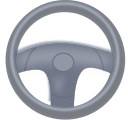
\includegraphics[width=0.7cm]{wheel.png}};
%\draw[thick,red] (3.5,-1.5) arc (0:50:1cm);

\end{scope}

%\begin{scope}[shift={(1,-5)}]
%\node (input0) at (4.5,0.00) [feature] {};
%\node (input1) at (4.5,0.20) [feature] {};
%\node (input2) at (4.5,0.40) [feature] {};
%\node (input3) at (4.5,0.60) [feature] {};
%\node (input4) at (4.5,0.80) [feature] {};
%\node (input5) at (4.5,1.00) [feature] {};
%\node (input6) at (4.5,1.20) [feature] {};
%\node (input7) at (4.5,1.40) [feature] {};
%\node (input8) at (4.5,1.60) [feature] {};
%\node (input9) at (4.5,1.80) [feature] {};
%\node (input10) at (4.5,2.00) [feature] {};
%\node (input11) at (4.5,2.20) [feature] {};
%\node (input12) at (4.5,2.40) [feature] {};
%\node (input13) at (4.5,2.60) [feature] {};
%\node (input14) at (4.5,2.80) [feature] {};
%\node (input15) at (4.5,3.00) [feature] {};
%\node (input16) at (4.5,3.20) [feature] {};
%\node (input17) at (4.5,3.40) [feature] {};
%\node (input18) at (4.5,3.60) [feature] {};
%\node (input19) at (4.5,3.80) [feature] {};
%\node (input20) at (4.5,4.00) [feature] {};
%\node (input21) at (4.5,4.20) [feature] {};
%\node (input22) at (4.5,4.40) [feature] {};
%\node (input23) at (4.5,4.60) [feature] {};
%\node (input24) at (4.5,4.80) [feature] {};
%\node (input25) at (4.5,5.00) [feature] {};
%\node (input26) at (4.5,5.20) [feature] {};
%\node (input27) at (4.5,5.40) [feature] {};
%\node (input28) at (4.5,5.60) [feature] {};
%\node (input29) at (4.5,5.80) [feature] {};
%\node (input30) at (4.5,6.00) [feature] {};
%\node (input31) at (4.5,6.20) [feature] {};
%\end{scope}

%\shade[right color=white!10!black,left color=white!50!black] (cfeat0.north east) -- (input3.north west) -- (input0.south west) -- (cfeat0.south east) ;
%\shade[right color=white!10!black,left color=white!50!black] (cfeat1.north east) -- (input7.north west) -- (input4.south west) -- (cfeat1.south east) ;
%\shade[right color=white!10!black,left color=white!50!black] (cfeat2.north east) -- (input11.north west) -- (input8.south west) -- (cfeat2.south east) ;
%\shade[right color=white!10!black,left color=white!50!black] (cfeat3.north east) -- (input15.north west) -- (input12.south west) -- (cfeat3.south east) ;
%\shade[right color=white!10!black,left color=white!50!black] (cfeat4.north east) -- (input19.north west) -- (input16.south west) -- (cfeat4.south east) ;
%\shade[right color=white!10!black,left color=white!50!black] (cfeat5.north east) -- (input23.north west) -- (input20.south west) -- (cfeat5.south east) ;
%\shade[right color=white!10!black,left color=white!50!black] (cfeat6.north east) -- (input27.north west) -- (input24.south west) -- (cfeat6.south east) ;
%\shade[right color=white!10!black,left color=white!50!black] (cfeat7.north east) -- (input31.north west) -- (input28.south west) -- (cfeat7.south east) ;



%\node at (5.0,1.60) [anchor=center,color=white] {\scriptsize{Sensory}};
\node at (6.3,1.60) [anchor=center,color=white] {\scriptsize{Fully-connected}};
\node at (8.3,1.60) [anchor=center,color=white] {\scriptsize{Fully-connected}};
\node at (9.8,1.60) [anchor=center,color=white] {\scriptsize{Motor}};
%\node at (5.0,1.40) [anchor=center,color=white] {\scriptsize{neurons}};
\node at (6.5,1.40) [anchor=center,color=white] {\scriptsize{layer \#1}};
\node at (8.3,1.40) [anchor=center,color=white] {\scriptsize{layer \#2}};
\node at (9.8,1.40) [anchor=center,color=white] {\scriptsize{neurons}};

% Command to motor
\begin{scope}[shift={(5.6,-4.6)}]
\node (n0) at (0.00,0.00) [neuronart,fill=neur0] {};
\node (n1) at (0.09,0.00) [neuronart,fill=neur1] {};
\node (n2) at (0.18,0.00) [neuronart,fill=neur2] {};
\node (n3) at (0.27,0.00) [neuronart,fill=neur3] {};
\node (n4) at (0.36,0.00) [neuronart,fill=neur4] {};
\node (n5) at (0.45,0.00) [neuronart,fill=neur5] {};
\node (n6) at (0.54,0.00) [neuronart,fill=neur6] {};
\node (n7) at (0.63,0.00) [neuronart,fill=neur7] {};
\node (n8) at (0.72,0.00) [neuronart,fill=neur8] {};
\node (n9) at (0.81,0.00) [neuronart,fill=neur9] {};
\node (n10) at (0.90,0.00) [neuronart,fill=neur10] {};
\node (n11) at (0.99,0.00) [neuronart,fill=neur11] {};
\node (n12) at (1.08,0.00) [neuronart,fill=neur12] {};
\node (n13) at (1.17,0.00) [neuronart,fill=neur13] {};
\node (n14) at (1.26,0.00) [neuronart,fill=neur14] {};
\node (n15) at (1.35,0.00) [neuronart,fill=neur15] {};
\node (n16) at (1.44,0.00) [neuronart,fill=neur16] {};
\node (n17) at (1.53,0.00) [neuronart,fill=neur17] {};
\node (n18) at (1.62,0.00) [neuronart,fill=neur18] {};
\node (n19) at (1.71,0.00) [neuronart,fill=neur19] {};
\node (n20) at (0.00,0.11) [neuronart,fill=neur20] {};
\node (n21) at (0.09,0.11) [neuronart,fill=neur21] {};
\node (n22) at (0.18,0.11) [neuronart,fill=neur22] {};
\node (n23) at (0.27,0.11) [neuronart,fill=neur23] {};
\node (n24) at (0.36,0.11) [neuronart,fill=neur24] {};
\node (n25) at (0.45,0.11) [neuronart,fill=neur25] {};
\node (n26) at (0.54,0.11) [neuronart,fill=neur26] {};
\node (n27) at (0.63,0.11) [neuronart,fill=neur27] {};
\node (n28) at (0.72,0.11) [neuronart,fill=neur28] {};
\node (n29) at (0.81,0.11) [neuronart,fill=neur29] {};
\node (n30) at (0.90,0.11) [neuronart,fill=neur30] {};
\node (n31) at (0.99,0.11) [neuronart,fill=neur31] {};
\node (n32) at (1.08,0.11) [neuronart,fill=neur32] {};
\node (n33) at (1.17,0.11) [neuronart,fill=neur33] {};
\node (n34) at (1.26,0.11) [neuronart,fill=neur34] {};
\node (n35) at (1.35,0.11) [neuronart,fill=neur35] {};
\node (n36) at (1.44,0.11) [neuronart,fill=neur36] {};
\node (n37) at (1.53,0.11) [neuronart,fill=neur37] {};
\node (n38) at (1.62,0.11) [neuronart,fill=neur38] {};
\node (n39) at (1.71,0.11) [neuronart,fill=neur39] {};
\node (n40) at (0.00,0.23) [neuronart,fill=neur40] {};
\node (n41) at (0.09,0.23) [neuronart,fill=neur41] {};
\node (n42) at (0.18,0.23) [neuronart,fill=neur42] {};
\node (n43) at (0.27,0.23) [neuronart,fill=neur43] {};
\node (n44) at (0.36,0.23) [neuronart,fill=neur44] {};
\node (n45) at (0.45,0.23) [neuronart,fill=neur45] {};
\node (n46) at (0.54,0.23) [neuronart,fill=neur46] {};
\node (n47) at (0.63,0.23) [neuronart,fill=neur47] {};
\node (n48) at (0.72,0.23) [neuronart,fill=neur48] {};
\node (n49) at (0.81,0.23) [neuronart,fill=neur49] {};
\node (n50) at (0.90,0.23) [neuronart,fill=neur50] {};
\node (n51) at (0.99,0.23) [neuronart,fill=neur51] {};
\node (n52) at (1.08,0.23) [neuronart,fill=neur52] {};
\node (n53) at (1.17,0.23) [neuronart,fill=neur53] {};
\node (n54) at (1.26,0.23) [neuronart,fill=neur54] {};
\node (n55) at (1.35,0.23) [neuronart,fill=neur55] {};
\node (n56) at (1.44,0.23) [neuronart,fill=neur56] {};
\node (n57) at (1.53,0.23) [neuronart,fill=neur57] {};
\node (n58) at (1.62,0.23) [neuronart,fill=neur58] {};
\node (n59) at (1.71,0.23) [neuronart,fill=neur59] {};
\node (n60) at (0.00,0.34) [neuronart,fill=neur60] {};
\node (n61) at (0.09,0.34) [neuronart,fill=neur61] {};
\node (n62) at (0.18,0.34) [neuronart,fill=neur62] {};
\node (n63) at (0.27,0.34) [neuronart,fill=neur63] {};
\node (n64) at (0.36,0.34) [neuronart,fill=neur64] {};
\node (n65) at (0.45,0.34) [neuronart,fill=neur65] {};
\node (n66) at (0.54,0.34) [neuronart,fill=neur66] {};
\node (n67) at (0.63,0.34) [neuronart,fill=neur67] {};
\node (n68) at (0.72,0.34) [neuronart,fill=neur68] {};
\node (n69) at (0.81,0.34) [neuronart,fill=neur69] {};
\node (n70) at (0.90,0.34) [neuronart,fill=neur70] {};
\node (n71) at (0.99,0.34) [neuronart,fill=neur71] {};
\node (n72) at (1.08,0.34) [neuronart,fill=neur72] {};
\node (n73) at (1.17,0.34) [neuronart,fill=neur73] {};
\node (n74) at (1.26,0.34) [neuronart,fill=neur74] {};
\node (n75) at (1.35,0.34) [neuronart,fill=neur75] {};
\node (n76) at (1.44,0.34) [neuronart,fill=neur76] {};
\node (n77) at (1.53,0.34) [neuronart,fill=neur77] {};
\node (n78) at (1.62,0.34) [neuronart,fill=neur78] {};
\node (n79) at (1.71,0.34) [neuronart,fill=neur79] {};
\node (n80) at (0.00,0.46) [neuronart,fill=neur80] {};
\node (n81) at (0.09,0.46) [neuronart,fill=neur81] {};
\node (n82) at (0.18,0.46) [neuronart,fill=neur82] {};
\node (n83) at (0.27,0.46) [neuronart,fill=neur83] {};
\node (n84) at (0.36,0.46) [neuronart,fill=neur84] {};
\node (n85) at (0.45,0.46) [neuronart,fill=neur85] {};
\node (n86) at (0.54,0.46) [neuronart,fill=neur86] {};
\node (n87) at (0.63,0.46) [neuronart,fill=neur87] {};
\node (n88) at (0.72,0.46) [neuronart,fill=neur88] {};
\node (n89) at (0.81,0.46) [neuronart,fill=neur89] {};
\node (n90) at (0.90,0.46) [neuronart,fill=neur90] {};
\node (n91) at (0.99,0.46) [neuronart,fill=neur91] {};
\node (n92) at (1.08,0.46) [neuronart,fill=neur92] {};
\node (n93) at (1.17,0.46) [neuronart,fill=neur93] {};
\node (n94) at (1.26,0.46) [neuronart,fill=neur94] {};
\node (n95) at (1.35,0.46) [neuronart,fill=neur95] {};
\node (n96) at (1.44,0.46) [neuronart,fill=neur96] {};
\node (n97) at (1.53,0.46) [neuronart,fill=neur97] {};
\node (n98) at (1.62,0.46) [neuronart,fill=neur98] {};
\node (n99) at (1.71,0.46) [neuronart,fill=neur99] {};
\node (n100) at (0.00,0.57) [neuronart,fill=neur100] {};
\node (n101) at (0.09,0.57) [neuronart,fill=neur101] {};
\node (n102) at (0.18,0.57) [neuronart,fill=neur102] {};
\node (n103) at (0.27,0.57) [neuronart,fill=neur103] {};
\node (n104) at (0.36,0.57) [neuronart,fill=neur104] {};
\node (n105) at (0.45,0.57) [neuronart,fill=neur105] {};
\node (n106) at (0.54,0.57) [neuronart,fill=neur106] {};
\node (n107) at (0.63,0.57) [neuronart,fill=neur107] {};
\node (n108) at (0.72,0.57) [neuronart,fill=neur108] {};
\node (n109) at (0.81,0.57) [neuronart,fill=neur109] {};
\node (n110) at (0.90,0.57) [neuronart,fill=neur110] {};
\node (n111) at (0.99,0.57) [neuronart,fill=neur111] {};
\node (n112) at (1.08,0.57) [neuronart,fill=neur112] {};
\node (n113) at (1.17,0.57) [neuronart,fill=neur113] {};
\node (n114) at (1.26,0.57) [neuronart,fill=neur114] {};
\node (n115) at (1.35,0.57) [neuronart,fill=neur115] {};
\node (n116) at (1.44,0.57) [neuronart,fill=neur116] {};
\node (n117) at (1.53,0.57) [neuronart,fill=neur117] {};
\node (n118) at (1.62,0.57) [neuronart,fill=neur118] {};
\node (n119) at (1.71,0.57) [neuronart,fill=neur119] {};
\node (n120) at (0.00,0.68) [neuronart,fill=neur120] {};
\node (n121) at (0.09,0.68) [neuronart,fill=neur121] {};
\node (n122) at (0.18,0.68) [neuronart,fill=neur122] {};
\node (n123) at (0.27,0.68) [neuronart,fill=neur123] {};
\node (n124) at (0.36,0.68) [neuronart,fill=neur124] {};
\node (n125) at (0.45,0.68) [neuronart,fill=neur125] {};
\node (n126) at (0.54,0.68) [neuronart,fill=neur126] {};
\node (n127) at (0.63,0.68) [neuronart,fill=neur127] {};
\node (n128) at (0.72,0.68) [neuronart,fill=neur128] {};
\node (n129) at (0.81,0.68) [neuronart,fill=neur129] {};
\node (n130) at (0.90,0.68) [neuronart,fill=neur130] {};
\node (n131) at (0.99,0.68) [neuronart,fill=neur131] {};
\node (n132) at (1.08,0.68) [neuronart,fill=neur132] {};
\node (n133) at (1.17,0.68) [neuronart,fill=neur133] {};
\node (n134) at (1.26,0.68) [neuronart,fill=neur134] {};
\node (n135) at (1.35,0.68) [neuronart,fill=neur135] {};
\node (n136) at (1.44,0.68) [neuronart,fill=neur136] {};
\node (n137) at (1.53,0.68) [neuronart,fill=neur137] {};
\node (n138) at (1.62,0.68) [neuronart,fill=neur138] {};
\node (n139) at (1.71,0.68) [neuronart,fill=neur139] {};
\node (n140) at (0.00,0.80) [neuronart,fill=neur140] {};
\node (n141) at (0.09,0.80) [neuronart,fill=neur141] {};
\node (n142) at (0.18,0.80) [neuronart,fill=neur142] {};
\node (n143) at (0.27,0.80) [neuronart,fill=neur143] {};
\node (n144) at (0.36,0.80) [neuronart,fill=neur144] {};
\node (n145) at (0.45,0.80) [neuronart,fill=neur145] {};
\node (n146) at (0.54,0.80) [neuronart,fill=neur146] {};
\node (n147) at (0.63,0.80) [neuronart,fill=neur147] {};
\node (n148) at (0.72,0.80) [neuronart,fill=neur148] {};
\node (n149) at (0.81,0.80) [neuronart,fill=neur149] {};
\node (n150) at (0.90,0.80) [neuronart,fill=neur150] {};
\node (n151) at (0.99,0.80) [neuronart,fill=neur151] {};
\node (n152) at (1.08,0.80) [neuronart,fill=neur152] {};
\node (n153) at (1.17,0.80) [neuronart,fill=neur153] {};
\node (n154) at (1.26,0.80) [neuronart,fill=neur154] {};
\node (n155) at (1.35,0.80) [neuronart,fill=neur155] {};
\node (n156) at (1.44,0.80) [neuronart,fill=neur156] {};
\node (n157) at (1.53,0.80) [neuronart,fill=neur157] {};
\node (n158) at (1.62,0.80) [neuronart,fill=neur158] {};
\node (n159) at (1.71,0.80) [neuronart,fill=neur159] {};
\node (n160) at (0.00,0.91) [neuronart,fill=neur160] {};
\node (n161) at (0.09,0.91) [neuronart,fill=neur161] {};
\node (n162) at (0.18,0.91) [neuronart,fill=neur162] {};
\node (n163) at (0.27,0.91) [neuronart,fill=neur163] {};
\node (n164) at (0.36,0.91) [neuronart,fill=neur164] {};
\node (n165) at (0.45,0.91) [neuronart,fill=neur165] {};
\node (n166) at (0.54,0.91) [neuronart,fill=neur166] {};
\node (n167) at (0.63,0.91) [neuronart,fill=neur167] {};
\node (n168) at (0.72,0.91) [neuronart,fill=neur168] {};
\node (n169) at (0.81,0.91) [neuronart,fill=neur169] {};
\node (n170) at (0.90,0.91) [neuronart,fill=neur170] {};
\node (n171) at (0.99,0.91) [neuronart,fill=neur171] {};
\node (n172) at (1.08,0.91) [neuronart,fill=neur172] {};
\node (n173) at (1.17,0.91) [neuronart,fill=neur173] {};
\node (n174) at (1.26,0.91) [neuronart,fill=neur174] {};
\node (n175) at (1.35,0.91) [neuronart,fill=neur175] {};
\node (n176) at (1.44,0.91) [neuronart,fill=neur176] {};
\node (n177) at (1.53,0.91) [neuronart,fill=neur177] {};
\node (n178) at (1.62,0.91) [neuronart,fill=neur178] {};
\node (n179) at (1.71,0.91) [neuronart,fill=neur179] {};
\node (n180) at (0.00,1.03) [neuronart,fill=neur180] {};
\node (n181) at (0.09,1.03) [neuronart,fill=neur181] {};
\node (n182) at (0.18,1.03) [neuronart,fill=neur182] {};
\node (n183) at (0.27,1.03) [neuronart,fill=neur183] {};
\node (n184) at (0.36,1.03) [neuronart,fill=neur184] {};
\node (n185) at (0.45,1.03) [neuronart,fill=neur185] {};
\node (n186) at (0.54,1.03) [neuronart,fill=neur186] {};
\node (n187) at (0.63,1.03) [neuronart,fill=neur187] {};
\node (n188) at (0.72,1.03) [neuronart,fill=neur188] {};
\node (n189) at (0.81,1.03) [neuronart,fill=neur189] {};
\node (n190) at (0.90,1.03) [neuronart,fill=neur190] {};
\node (n191) at (0.99,1.03) [neuronart,fill=neur191] {};
\node (n192) at (1.08,1.03) [neuronart,fill=neur192] {};
\node (n193) at (1.17,1.03) [neuronart,fill=neur193] {};
\node (n194) at (1.26,1.03) [neuronart,fill=neur194] {};
\node (n195) at (1.35,1.03) [neuronart,fill=neur195] {};
\node (n196) at (1.44,1.03) [neuronart,fill=neur196] {};
\node (n197) at (1.53,1.03) [neuronart,fill=neur197] {};
\node (n198) at (1.62,1.03) [neuronart,fill=neur198] {};
\node (n199) at (1.71,1.03) [neuronart,fill=neur199] {};
\node (n200) at (0.00,1.14) [neuronart,fill=neur200] {};
\node (n201) at (0.09,1.14) [neuronart,fill=neur201] {};
\node (n202) at (0.18,1.14) [neuronart,fill=neur202] {};
\node (n203) at (0.27,1.14) [neuronart,fill=neur203] {};
\node (n204) at (0.36,1.14) [neuronart,fill=neur204] {};
\node (n205) at (0.45,1.14) [neuronart,fill=neur205] {};
\node (n206) at (0.54,1.14) [neuronart,fill=neur206] {};
\node (n207) at (0.63,1.14) [neuronart,fill=neur207] {};
\node (n208) at (0.72,1.14) [neuronart,fill=neur208] {};
\node (n209) at (0.81,1.14) [neuronart,fill=neur209] {};
\node (n210) at (0.90,1.14) [neuronart,fill=neur210] {};
\node (n211) at (0.99,1.14) [neuronart,fill=neur211] {};
\node (n212) at (1.08,1.14) [neuronart,fill=neur212] {};
\node (n213) at (1.17,1.14) [neuronart,fill=neur213] {};
\node (n214) at (1.26,1.14) [neuronart,fill=neur214] {};
\node (n215) at (1.35,1.14) [neuronart,fill=neur215] {};
\node (n216) at (1.44,1.14) [neuronart,fill=neur216] {};
\node (n217) at (1.53,1.14) [neuronart,fill=neur217] {};
\node (n218) at (1.62,1.14) [neuronart,fill=neur218] {};
\node (n219) at (1.71,1.14) [neuronart,fill=neur219] {};
\node (n220) at (0.00,1.25) [neuronart,fill=neur220] {};
\node (n221) at (0.09,1.25) [neuronart,fill=neur221] {};
\node (n222) at (0.18,1.25) [neuronart,fill=neur222] {};
\node (n223) at (0.27,1.25) [neuronart,fill=neur223] {};
\node (n224) at (0.36,1.25) [neuronart,fill=neur224] {};
\node (n225) at (0.45,1.25) [neuronart,fill=neur225] {};
\node (n226) at (0.54,1.25) [neuronart,fill=neur226] {};
\node (n227) at (0.63,1.25) [neuronart,fill=neur227] {};
\node (n228) at (0.72,1.25) [neuronart,fill=neur228] {};
\node (n229) at (0.81,1.25) [neuronart,fill=neur229] {};
\node (n230) at (0.90,1.25) [neuronart,fill=neur230] {};
\node (n231) at (0.99,1.25) [neuronart,fill=neur231] {};
\node (n232) at (1.08,1.25) [neuronart,fill=neur232] {};
\node (n233) at (1.17,1.25) [neuronart,fill=neur233] {};
\node (n234) at (1.26,1.25) [neuronart,fill=neur234] {};
\node (n235) at (1.35,1.25) [neuronart,fill=neur235] {};
\node (n236) at (1.44,1.25) [neuronart,fill=neur236] {};
\node (n237) at (1.53,1.25) [neuronart,fill=neur237] {};
\node (n238) at (1.62,1.25) [neuronart,fill=neur238] {};
\node (n239) at (1.71,1.25) [neuronart,fill=neur239] {};
\node (n240) at (0.00,1.37) [neuronart,fill=neur240] {};
\node (n241) at (0.09,1.37) [neuronart,fill=neur241] {};
\node (n242) at (0.18,1.37) [neuronart,fill=neur242] {};
\node (n243) at (0.27,1.37) [neuronart,fill=neur243] {};
\node (n244) at (0.36,1.37) [neuronart,fill=neur244] {};
\node (n245) at (0.45,1.37) [neuronart,fill=neur245] {};
\node (n246) at (0.54,1.37) [neuronart,fill=neur246] {};
\node (n247) at (0.63,1.37) [neuronart,fill=neur247] {};
\node (n248) at (0.72,1.37) [neuronart,fill=neur248] {};
\node (n249) at (0.81,1.37) [neuronart,fill=neur249] {};
\node (n250) at (0.90,1.37) [neuronart,fill=neur250] {};
\node (n251) at (0.99,1.37) [neuronart,fill=neur251] {};
\node (n252) at (1.08,1.37) [neuronart,fill=neur252] {};
\node (n253) at (1.17,1.37) [neuronart,fill=neur253] {};
\node (n254) at (1.26,1.37) [neuronart,fill=neur254] {};
\node (n255) at (1.35,1.37) [neuronart,fill=neur255] {};
\node (n256) at (1.44,1.37) [neuronart,fill=neur256] {};
\node (n257) at (1.53,1.37) [neuronart,fill=neur257] {};
\node (n258) at (1.62,1.37) [neuronart,fill=neur258] {};
\node (n259) at (1.71,1.37) [neuronart,fill=neur259] {};
\node (n260) at (0.00,1.48) [neuronart,fill=neur260] {};
\node (n261) at (0.09,1.48) [neuronart,fill=neur261] {};
\node (n262) at (0.18,1.48) [neuronart,fill=neur262] {};
\node (n263) at (0.27,1.48) [neuronart,fill=neur263] {};
\node (n264) at (0.36,1.48) [neuronart,fill=neur264] {};
\node (n265) at (0.45,1.48) [neuronart,fill=neur265] {};
\node (n266) at (0.54,1.48) [neuronart,fill=neur266] {};
\node (n267) at (0.63,1.48) [neuronart,fill=neur267] {};
\node (n268) at (0.72,1.48) [neuronart,fill=neur268] {};
\node (n269) at (0.81,1.48) [neuronart,fill=neur269] {};
\node (n270) at (0.90,1.48) [neuronart,fill=neur270] {};
\node (n271) at (0.99,1.48) [neuronart,fill=neur271] {};
\node (n272) at (1.08,1.48) [neuronart,fill=neur272] {};
\node (n273) at (1.17,1.48) [neuronart,fill=neur273] {};
\node (n274) at (1.26,1.48) [neuronart,fill=neur274] {};
\node (n275) at (1.35,1.48) [neuronart,fill=neur275] {};
\node (n276) at (1.44,1.48) [neuronart,fill=neur276] {};
\node (n277) at (1.53,1.48) [neuronart,fill=neur277] {};
\node (n278) at (1.62,1.48) [neuronart,fill=neur278] {};
\node (n279) at (1.71,1.48) [neuronart,fill=neur279] {};
\node (n280) at (0.00,1.60) [neuronart,fill=neur280] {};
\node (n281) at (0.09,1.60) [neuronart,fill=neur281] {};
\node (n282) at (0.18,1.60) [neuronart,fill=neur282] {};
\node (n283) at (0.27,1.60) [neuronart,fill=neur283] {};
\node (n284) at (0.36,1.60) [neuronart,fill=neur284] {};
\node (n285) at (0.45,1.60) [neuronart,fill=neur285] {};
\node (n286) at (0.54,1.60) [neuronart,fill=neur286] {};
\node (n287) at (0.63,1.60) [neuronart,fill=neur287] {};
\node (n288) at (0.72,1.60) [neuronart,fill=neur288] {};
\node (n289) at (0.81,1.60) [neuronart,fill=neur289] {};
\node (n290) at (0.90,1.60) [neuronart,fill=neur290] {};
\node (n291) at (0.99,1.60) [neuronart,fill=neur291] {};
\node (n292) at (1.08,1.60) [neuronart,fill=neur292] {};
\node (n293) at (1.17,1.60) [neuronart,fill=neur293] {};
\node (n294) at (1.26,1.60) [neuronart,fill=neur294] {};
\node (n295) at (1.35,1.60) [neuronart,fill=neur295] {};
\node (n296) at (1.44,1.60) [neuronart,fill=neur296] {};
\node (n297) at (1.53,1.60) [neuronart,fill=neur297] {};
\node (n298) at (1.62,1.60) [neuronart,fill=neur298] {};
\node (n299) at (1.71,1.60) [neuronart,fill=neur299] {};
\node (n300) at (0.00,1.71) [neuronart,fill=neur300] {};
\node (n301) at (0.09,1.71) [neuronart,fill=neur301] {};
\node (n302) at (0.18,1.71) [neuronart,fill=neur302] {};
\node (n303) at (0.27,1.71) [neuronart,fill=neur303] {};
\node (n304) at (0.36,1.71) [neuronart,fill=neur304] {};
\node (n305) at (0.45,1.71) [neuronart,fill=neur305] {};
\node (n306) at (0.54,1.71) [neuronart,fill=neur306] {};
\node (n307) at (0.63,1.71) [neuronart,fill=neur307] {};
\node (n308) at (0.72,1.71) [neuronart,fill=neur308] {};
\node (n309) at (0.81,1.71) [neuronart,fill=neur309] {};
\node (n310) at (0.90,1.71) [neuronart,fill=neur310] {};
\node (n311) at (0.99,1.71) [neuronart,fill=neur311] {};
\node (n312) at (1.08,1.71) [neuronart,fill=neur312] {};
\node (n313) at (1.17,1.71) [neuronart,fill=neur313] {};
\node (n314) at (1.26,1.71) [neuronart,fill=neur314] {};
\node (n315) at (1.35,1.71) [neuronart,fill=neur315] {};
\node (n316) at (1.44,1.71) [neuronart,fill=neur316] {};
\node (n317) at (1.53,1.71) [neuronart,fill=neur317] {};
\node (n318) at (1.62,1.71) [neuronart,fill=neur318] {};
\node (n319) at (1.71,1.71) [neuronart,fill=neur319] {};
\node (n320) at (0.00,1.82) [neuronart,fill=neur320] {};
\node (n321) at (0.09,1.82) [neuronart,fill=neur321] {};
\node (n322) at (0.18,1.82) [neuronart,fill=neur322] {};
\node (n323) at (0.27,1.82) [neuronart,fill=neur323] {};
\node (n324) at (0.36,1.82) [neuronart,fill=neur324] {};
\node (n325) at (0.45,1.82) [neuronart,fill=neur325] {};
\node (n326) at (0.54,1.82) [neuronart,fill=neur326] {};
\node (n327) at (0.63,1.82) [neuronart,fill=neur327] {};
\node (n328) at (0.72,1.82) [neuronart,fill=neur328] {};
\node (n329) at (0.81,1.82) [neuronart,fill=neur329] {};
\node (n330) at (0.90,1.82) [neuronart,fill=neur330] {};
\node (n331) at (0.99,1.82) [neuronart,fill=neur331] {};
\node (n332) at (1.08,1.82) [neuronart,fill=neur332] {};
\node (n333) at (1.17,1.82) [neuronart,fill=neur333] {};
\node (n334) at (1.26,1.82) [neuronart,fill=neur334] {};
\node (n335) at (1.35,1.82) [neuronart,fill=neur335] {};
\node (n336) at (1.44,1.82) [neuronart,fill=neur336] {};
\node (n337) at (1.53,1.82) [neuronart,fill=neur337] {};
\node (n338) at (1.62,1.82) [neuronart,fill=neur338] {};
\node (n339) at (1.71,1.82) [neuronart,fill=neur339] {};
\node (n340) at (0.00,1.94) [neuronart,fill=neur340] {};
\node (n341) at (0.09,1.94) [neuronart,fill=neur341] {};
\node (n342) at (0.18,1.94) [neuronart,fill=neur342] {};
\node (n343) at (0.27,1.94) [neuronart,fill=neur343] {};
\node (n344) at (0.36,1.94) [neuronart,fill=neur344] {};
\node (n345) at (0.45,1.94) [neuronart,fill=neur345] {};
\node (n346) at (0.54,1.94) [neuronart,fill=neur346] {};
\node (n347) at (0.63,1.94) [neuronart,fill=neur347] {};
\node (n348) at (0.72,1.94) [neuronart,fill=neur348] {};
\node (n349) at (0.81,1.94) [neuronart,fill=neur349] {};
\node (n350) at (0.90,1.94) [neuronart,fill=neur350] {};
\node (n351) at (0.99,1.94) [neuronart,fill=neur351] {};
\node (n352) at (1.08,1.94) [neuronart,fill=neur352] {};
\node (n353) at (1.17,1.94) [neuronart,fill=neur353] {};
\node (n354) at (1.26,1.94) [neuronart,fill=neur354] {};
\node (n355) at (1.35,1.94) [neuronart,fill=neur355] {};
\node (n356) at (1.44,1.94) [neuronart,fill=neur356] {};
\node (n357) at (1.53,1.94) [neuronart,fill=neur357] {};
\node (n358) at (1.62,1.94) [neuronart,fill=neur358] {};
\node (n359) at (1.71,1.94) [neuronart,fill=neur359] {};
\node (n360) at (0.00,2.05) [neuronart,fill=neur360] {};
\node (n361) at (0.09,2.05) [neuronart,fill=neur361] {};
\node (n362) at (0.18,2.05) [neuronart,fill=neur362] {};
\node (n363) at (0.27,2.05) [neuronart,fill=neur363] {};
\node (n364) at (0.36,2.05) [neuronart,fill=neur364] {};
\node (n365) at (0.45,2.05) [neuronart,fill=neur365] {};
\node (n366) at (0.54,2.05) [neuronart,fill=neur366] {};
\node (n367) at (0.63,2.05) [neuronart,fill=neur367] {};
\node (n368) at (0.72,2.05) [neuronart,fill=neur368] {};
\node (n369) at (0.81,2.05) [neuronart,fill=neur369] {};
\node (n370) at (0.90,2.05) [neuronart,fill=neur370] {};
\node (n371) at (0.99,2.05) [neuronart,fill=neur371] {};
\node (n372) at (1.08,2.05) [neuronart,fill=neur372] {};
\node (n373) at (1.17,2.05) [neuronart,fill=neur373] {};
\node (n374) at (1.26,2.05) [neuronart,fill=neur374] {};
\node (n375) at (1.35,2.05) [neuronart,fill=neur375] {};
\node (n376) at (1.44,2.05) [neuronart,fill=neur376] {};
\node (n377) at (1.53,2.05) [neuronart,fill=neur377] {};
\node (n378) at (1.62,2.05) [neuronart,fill=neur378] {};
\node (n379) at (1.71,2.05) [neuronart,fill=neur379] {};
\node (n380) at (0.00,2.17) [neuronart,fill=neur380] {};
\node (n381) at (0.09,2.17) [neuronart,fill=neur381] {};
\node (n382) at (0.18,2.17) [neuronart,fill=neur382] {};
\node (n383) at (0.27,2.17) [neuronart,fill=neur383] {};
\node (n384) at (0.36,2.17) [neuronart,fill=neur384] {};
\node (n385) at (0.45,2.17) [neuronart,fill=neur385] {};
\node (n386) at (0.54,2.17) [neuronart,fill=neur386] {};
\node (n387) at (0.63,2.17) [neuronart,fill=neur387] {};
\node (n388) at (0.72,2.17) [neuronart,fill=neur388] {};
\node (n389) at (0.81,2.17) [neuronart,fill=neur389] {};
\node (n390) at (0.90,2.17) [neuronart,fill=neur390] {};
\node (n391) at (0.99,2.17) [neuronart,fill=neur391] {};
\node (n392) at (1.08,2.17) [neuronart,fill=neur392] {};
\node (n393) at (1.17,2.17) [neuronart,fill=neur393] {};
\node (n394) at (1.26,2.17) [neuronart,fill=neur394] {};
\node (n395) at (1.35,2.17) [neuronart,fill=neur395] {};
\node (n396) at (1.44,2.17) [neuronart,fill=neur396] {};
\node (n397) at (1.53,2.17) [neuronart,fill=neur397] {};
\node (n398) at (1.62,2.17) [neuronart,fill=neur398] {};
\node (n399) at (1.71,2.17) [neuronart,fill=neur399] {};
\node (n400) at (0.00,2.28) [neuronart,fill=neur400] {};
\node (n401) at (0.09,2.28) [neuronart,fill=neur401] {};
\node (n402) at (0.18,2.28) [neuronart,fill=neur402] {};
\node (n403) at (0.27,2.28) [neuronart,fill=neur403] {};
\node (n404) at (0.36,2.28) [neuronart,fill=neur404] {};
\node (n405) at (0.45,2.28) [neuronart,fill=neur405] {};
\node (n406) at (0.54,2.28) [neuronart,fill=neur406] {};
\node (n407) at (0.63,2.28) [neuronart,fill=neur407] {};
\node (n408) at (0.72,2.28) [neuronart,fill=neur408] {};
\node (n409) at (0.81,2.28) [neuronart,fill=neur409] {};
\node (n410) at (0.90,2.28) [neuronart,fill=neur410] {};
\node (n411) at (0.99,2.28) [neuronart,fill=neur411] {};
\node (n412) at (1.08,2.28) [neuronart,fill=neur412] {};
\node (n413) at (1.17,2.28) [neuronart,fill=neur413] {};
\node (n414) at (1.26,2.28) [neuronart,fill=neur414] {};
\node (n415) at (1.35,2.28) [neuronart,fill=neur415] {};
\node (n416) at (1.44,2.28) [neuronart,fill=neur416] {};
\node (n417) at (1.53,2.28) [neuronart,fill=neur417] {};
\node (n418) at (1.62,2.28) [neuronart,fill=neur418] {};
\node (n419) at (1.71,2.28) [neuronart,fill=neur419] {};
\node (n420) at (0.00,2.39) [neuronart,fill=neur420] {};
\node (n421) at (0.09,2.39) [neuronart,fill=neur421] {};
\node (n422) at (0.18,2.39) [neuronart,fill=neur422] {};
\node (n423) at (0.27,2.39) [neuronart,fill=neur423] {};
\node (n424) at (0.36,2.39) [neuronart,fill=neur424] {};
\node (n425) at (0.45,2.39) [neuronart,fill=neur425] {};
\node (n426) at (0.54,2.39) [neuronart,fill=neur426] {};
\node (n427) at (0.63,2.39) [neuronart,fill=neur427] {};
\node (n428) at (0.72,2.39) [neuronart,fill=neur428] {};
\node (n429) at (0.81,2.39) [neuronart,fill=neur429] {};
\node (n430) at (0.90,2.39) [neuronart,fill=neur430] {};
\node (n431) at (0.99,2.39) [neuronart,fill=neur431] {};
\node (n432) at (1.08,2.39) [neuronart,fill=neur432] {};
\node (n433) at (1.17,2.39) [neuronart,fill=neur433] {};
\node (n434) at (1.26,2.39) [neuronart,fill=neur434] {};
\node (n435) at (1.35,2.39) [neuronart,fill=neur435] {};
\node (n436) at (1.44,2.39) [neuronart,fill=neur436] {};
\node (n437) at (1.53,2.39) [neuronart,fill=neur437] {};
\node (n438) at (1.62,2.39) [neuronart,fill=neur438] {};
\node (n439) at (1.71,2.39) [neuronart,fill=neur439] {};
\node (n440) at (0.00,2.51) [neuronart,fill=neur440] {};
\node (n441) at (0.09,2.51) [neuronart,fill=neur441] {};
\node (n442) at (0.18,2.51) [neuronart,fill=neur442] {};
\node (n443) at (0.27,2.51) [neuronart,fill=neur443] {};
\node (n444) at (0.36,2.51) [neuronart,fill=neur444] {};
\node (n445) at (0.45,2.51) [neuronart,fill=neur445] {};
\node (n446) at (0.54,2.51) [neuronart,fill=neur446] {};
\node (n447) at (0.63,2.51) [neuronart,fill=neur447] {};
\node (n448) at (0.72,2.51) [neuronart,fill=neur448] {};
\node (n449) at (0.81,2.51) [neuronart,fill=neur449] {};
\node (n450) at (0.90,2.51) [neuronart,fill=neur450] {};
\node (n451) at (0.99,2.51) [neuronart,fill=neur451] {};
\node (n452) at (1.08,2.51) [neuronart,fill=neur452] {};
\node (n453) at (1.17,2.51) [neuronart,fill=neur453] {};
\node (n454) at (1.26,2.51) [neuronart,fill=neur454] {};
\node (n455) at (1.35,2.51) [neuronart,fill=neur455] {};
\node (n456) at (1.44,2.51) [neuronart,fill=neur456] {};
\node (n457) at (1.53,2.51) [neuronart,fill=neur457] {};
\node (n458) at (1.62,2.51) [neuronart,fill=neur458] {};
\node (n459) at (1.71,2.51) [neuronart,fill=neur459] {};
\node (n460) at (0.00,2.62) [neuronart,fill=neur460] {};
\node (n461) at (0.09,2.62) [neuronart,fill=neur461] {};
\node (n462) at (0.18,2.62) [neuronart,fill=neur462] {};
\node (n463) at (0.27,2.62) [neuronart,fill=neur463] {};
\node (n464) at (0.36,2.62) [neuronart,fill=neur464] {};
\node (n465) at (0.45,2.62) [neuronart,fill=neur465] {};
\node (n466) at (0.54,2.62) [neuronart,fill=neur466] {};
\node (n467) at (0.63,2.62) [neuronart,fill=neur467] {};
\node (n468) at (0.72,2.62) [neuronart,fill=neur468] {};
\node (n469) at (0.81,2.62) [neuronart,fill=neur469] {};
\node (n470) at (0.90,2.62) [neuronart,fill=neur470] {};
\node (n471) at (0.99,2.62) [neuronart,fill=neur471] {};
\node (n472) at (1.08,2.62) [neuronart,fill=neur472] {};
\node (n473) at (1.17,2.62) [neuronart,fill=neur473] {};
\node (n474) at (1.26,2.62) [neuronart,fill=neur474] {};
\node (n475) at (1.35,2.62) [neuronart,fill=neur475] {};
\node (n476) at (1.44,2.62) [neuronart,fill=neur476] {};
\node (n477) at (1.53,2.62) [neuronart,fill=neur477] {};
\node (n478) at (1.62,2.62) [neuronart,fill=neur478] {};
\node (n479) at (1.71,2.62) [neuronart,fill=neur479] {};
\node (n480) at (0.00,2.74) [neuronart,fill=neur480] {};
\node (n481) at (0.09,2.74) [neuronart,fill=neur481] {};
\node (n482) at (0.18,2.74) [neuronart,fill=neur482] {};
\node (n483) at (0.27,2.74) [neuronart,fill=neur483] {};
\node (n484) at (0.36,2.74) [neuronart,fill=neur484] {};
\node (n485) at (0.45,2.74) [neuronart,fill=neur485] {};
\node (n486) at (0.54,2.74) [neuronart,fill=neur486] {};
\node (n487) at (0.63,2.74) [neuronart,fill=neur487] {};
\node (n488) at (0.72,2.74) [neuronart,fill=neur488] {};
\node (n489) at (0.81,2.74) [neuronart,fill=neur489] {};
\node (n490) at (0.90,2.74) [neuronart,fill=neur490] {};
\node (n491) at (0.99,2.74) [neuronart,fill=neur491] {};
\node (n492) at (1.08,2.74) [neuronart,fill=neur492] {};
\node (n493) at (1.17,2.74) [neuronart,fill=neur493] {};
\node (n494) at (1.26,2.74) [neuronart,fill=neur494] {};
\node (n495) at (1.35,2.74) [neuronart,fill=neur495] {};
\node (n496) at (1.44,2.74) [neuronart,fill=neur496] {};
\node (n497) at (1.53,2.74) [neuronart,fill=neur497] {};
\node (n498) at (1.62,2.74) [neuronart,fill=neur498] {};
\node (n499) at (1.71,2.74) [neuronart,fill=neur499] {};
\node (n500) at (0.00,2.85) [neuronart,fill=neur500] {};
\node (n501) at (0.09,2.85) [neuronart,fill=neur501] {};
\node (n502) at (0.18,2.85) [neuronart,fill=neur502] {};
\node (n503) at (0.27,2.85) [neuronart,fill=neur503] {};
\node (n504) at (0.36,2.85) [neuronart,fill=neur504] {};
\node (n505) at (0.45,2.85) [neuronart,fill=neur505] {};
\node (n506) at (0.54,2.85) [neuronart,fill=neur506] {};
\node (n507) at (0.63,2.85) [neuronart,fill=neur507] {};
\node (n508) at (0.72,2.85) [neuronart,fill=neur508] {};
\node (n509) at (0.81,2.85) [neuronart,fill=neur509] {};
\node (n510) at (0.90,2.85) [neuronart,fill=neur510] {};
\node (n511) at (0.99,2.85) [neuronart,fill=neur511] {};
\node (n512) at (1.08,2.85) [neuronart,fill=neur512] {};
\node (n513) at (1.17,2.85) [neuronart,fill=neur513] {};
\node (n514) at (1.26,2.85) [neuronart,fill=neur514] {};
\node (n515) at (1.35,2.85) [neuronart,fill=neur515] {};
\node (n516) at (1.44,2.85) [neuronart,fill=neur516] {};
\node (n517) at (1.53,2.85) [neuronart,fill=neur517] {};
\node (n518) at (1.62,2.85) [neuronart,fill=neur518] {};
\node (n519) at (1.71,2.85) [neuronart,fill=neur519] {};
\node (n520) at (0.00,2.96) [neuronart,fill=neur520] {};
\node (n521) at (0.09,2.96) [neuronart,fill=neur521] {};
\node (n522) at (0.18,2.96) [neuronart,fill=neur522] {};
\node (n523) at (0.27,2.96) [neuronart,fill=neur523] {};
\node (n524) at (0.36,2.96) [neuronart,fill=neur524] {};
\node (n525) at (0.45,2.96) [neuronart,fill=neur525] {};
\node (n526) at (0.54,2.96) [neuronart,fill=neur526] {};
\node (n527) at (0.63,2.96) [neuronart,fill=neur527] {};
\node (n528) at (0.72,2.96) [neuronart,fill=neur528] {};
\node (n529) at (0.81,2.96) [neuronart,fill=neur529] {};
\node (n530) at (0.90,2.96) [neuronart,fill=neur530] {};
\node (n531) at (0.99,2.96) [neuronart,fill=neur531] {};
\node (n532) at (1.08,2.96) [neuronart,fill=neur532] {};
\node (n533) at (1.17,2.96) [neuronart,fill=neur533] {};
\node (n534) at (1.26,2.96) [neuronart,fill=neur534] {};
\node (n535) at (1.35,2.96) [neuronart,fill=neur535] {};
\node (n536) at (1.44,2.96) [neuronart,fill=neur536] {};
\node (n537) at (1.53,2.96) [neuronart,fill=neur537] {};
\node (n538) at (1.62,2.96) [neuronart,fill=neur538] {};
\node (n539) at (1.71,2.96) [neuronart,fill=neur539] {};
\node (n540) at (0.00,3.08) [neuronart,fill=neur540] {};
\node (n541) at (0.09,3.08) [neuronart,fill=neur541] {};
\node (n542) at (0.18,3.08) [neuronart,fill=neur542] {};
\node (n543) at (0.27,3.08) [neuronart,fill=neur543] {};
\node (n544) at (0.36,3.08) [neuronart,fill=neur544] {};
\node (n545) at (0.45,3.08) [neuronart,fill=neur545] {};
\node (n546) at (0.54,3.08) [neuronart,fill=neur546] {};
\node (n547) at (0.63,3.08) [neuronart,fill=neur547] {};
\node (n548) at (0.72,3.08) [neuronart,fill=neur548] {};
\node (n549) at (0.81,3.08) [neuronart,fill=neur549] {};
\node (n550) at (0.90,3.08) [neuronart,fill=neur550] {};
\node (n551) at (0.99,3.08) [neuronart,fill=neur551] {};
\node (n552) at (1.08,3.08) [neuronart,fill=neur552] {};
\node (n553) at (1.17,3.08) [neuronart,fill=neur553] {};
\node (n554) at (1.26,3.08) [neuronart,fill=neur554] {};
\node (n555) at (1.35,3.08) [neuronart,fill=neur555] {};
\node (n556) at (1.44,3.08) [neuronart,fill=neur556] {};
\node (n557) at (1.53,3.08) [neuronart,fill=neur557] {};
\node (n558) at (1.62,3.08) [neuronart,fill=neur558] {};
\node (n559) at (1.71,3.08) [neuronart,fill=neur559] {};
\node (n560) at (0.00,3.19) [neuronart,fill=neur560] {};
\node (n561) at (0.09,3.19) [neuronart,fill=neur561] {};
\node (n562) at (0.18,3.19) [neuronart,fill=neur562] {};
\node (n563) at (0.27,3.19) [neuronart,fill=neur563] {};
\node (n564) at (0.36,3.19) [neuronart,fill=neur564] {};
\node (n565) at (0.45,3.19) [neuronart,fill=neur565] {};
\node (n566) at (0.54,3.19) [neuronart,fill=neur566] {};
\node (n567) at (0.63,3.19) [neuronart,fill=neur567] {};
\node (n568) at (0.72,3.19) [neuronart,fill=neur568] {};
\node (n569) at (0.81,3.19) [neuronart,fill=neur569] {};
\node (n570) at (0.90,3.19) [neuronart,fill=neur570] {};
\node (n571) at (0.99,3.19) [neuronart,fill=neur571] {};
\node (n572) at (1.08,3.19) [neuronart,fill=neur572] {};
\node (n573) at (1.17,3.19) [neuronart,fill=neur573] {};
\node (n574) at (1.26,3.19) [neuronart,fill=neur574] {};
\node (n575) at (1.35,3.19) [neuronart,fill=neur575] {};
\node (n576) at (1.44,3.19) [neuronart,fill=neur576] {};
\node (n577) at (1.53,3.19) [neuronart,fill=neur577] {};
\node (n578) at (1.62,3.19) [neuronart,fill=neur578] {};
\node (n579) at (1.71,3.19) [neuronart,fill=neur579] {};
\node (n580) at (0.00,3.31) [neuronart,fill=neur580] {};
\node (n581) at (0.09,3.31) [neuronart,fill=neur581] {};
\node (n582) at (0.18,3.31) [neuronart,fill=neur582] {};
\node (n583) at (0.27,3.31) [neuronart,fill=neur583] {};
\node (n584) at (0.36,3.31) [neuronart,fill=neur584] {};
\node (n585) at (0.45,3.31) [neuronart,fill=neur585] {};
\node (n586) at (0.54,3.31) [neuronart,fill=neur586] {};
\node (n587) at (0.63,3.31) [neuronart,fill=neur587] {};
\node (n588) at (0.72,3.31) [neuronart,fill=neur588] {};
\node (n589) at (0.81,3.31) [neuronart,fill=neur589] {};
\node (n590) at (0.90,3.31) [neuronart,fill=neur590] {};
\node (n591) at (0.99,3.31) [neuronart,fill=neur591] {};
\node (n592) at (1.08,3.31) [neuronart,fill=neur592] {};
\node (n593) at (1.17,3.31) [neuronart,fill=neur593] {};
\node (n594) at (1.26,3.31) [neuronart,fill=neur594] {};
\node (n595) at (1.35,3.31) [neuronart,fill=neur595] {};
\node (n596) at (1.44,3.31) [neuronart,fill=neur596] {};
\node (n597) at (1.53,3.31) [neuronart,fill=neur597] {};
\node (n598) at (1.62,3.31) [neuronart,fill=neur598] {};
\node (n599) at (1.71,3.31) [neuronart,fill=neur599] {};
\node (n600) at (0.00,3.42) [neuronart,fill=neur600] {};
\node (n601) at (0.09,3.42) [neuronart,fill=neur601] {};
\node (n602) at (0.18,3.42) [neuronart,fill=neur602] {};
\node (n603) at (0.27,3.42) [neuronart,fill=neur603] {};
\node (n604) at (0.36,3.42) [neuronart,fill=neur604] {};
\node (n605) at (0.45,3.42) [neuronart,fill=neur605] {};
\node (n606) at (0.54,3.42) [neuronart,fill=neur606] {};
\node (n607) at (0.63,3.42) [neuronart,fill=neur607] {};
\node (n608) at (0.72,3.42) [neuronart,fill=neur608] {};
\node (n609) at (0.81,3.42) [neuronart,fill=neur609] {};
\node (n610) at (0.90,3.42) [neuronart,fill=neur610] {};
\node (n611) at (0.99,3.42) [neuronart,fill=neur611] {};
\node (n612) at (1.08,3.42) [neuronart,fill=neur612] {};
\node (n613) at (1.17,3.42) [neuronart,fill=neur613] {};
\node (n614) at (1.26,3.42) [neuronart,fill=neur614] {};
\node (n615) at (1.35,3.42) [neuronart,fill=neur615] {};
\node (n616) at (1.44,3.42) [neuronart,fill=neur616] {};
\node (n617) at (1.53,3.42) [neuronart,fill=neur617] {};
\node (n618) at (1.62,3.42) [neuronart,fill=neur618] {};
\node (n619) at (1.71,3.42) [neuronart,fill=neur619] {};
\node (n620) at (0.00,3.53) [neuronart,fill=neur620] {};
\node (n621) at (0.09,3.53) [neuronart,fill=neur621] {};
\node (n622) at (0.18,3.53) [neuronart,fill=neur622] {};
\node (n623) at (0.27,3.53) [neuronart,fill=neur623] {};
\node (n624) at (0.36,3.53) [neuronart,fill=neur624] {};
\node (n625) at (0.45,3.53) [neuronart,fill=neur625] {};
\node (n626) at (0.54,3.53) [neuronart,fill=neur626] {};
\node (n627) at (0.63,3.53) [neuronart,fill=neur627] {};
\node (n628) at (0.72,3.53) [neuronart,fill=neur628] {};
\node (n629) at (0.81,3.53) [neuronart,fill=neur629] {};
\node (n630) at (0.90,3.53) [neuronart,fill=neur630] {};
\node (n631) at (0.99,3.53) [neuronart,fill=neur631] {};
\node (n632) at (1.08,3.53) [neuronart,fill=neur632] {};
\node (n633) at (1.17,3.53) [neuronart,fill=neur633] {};
\node (n634) at (1.26,3.53) [neuronart,fill=neur634] {};
\node (n635) at (1.35,3.53) [neuronart,fill=neur635] {};
\node (n636) at (1.44,3.53) [neuronart,fill=neur636] {};
\node (n637) at (1.53,3.53) [neuronart,fill=neur637] {};
\node (n638) at (1.62,3.53) [neuronart,fill=neur638] {};
\node (n639) at (1.71,3.53) [neuronart,fill=neur639] {};
\node (n640) at (0.00,3.65) [neuronart,fill=neur640] {};
\node (n641) at (0.09,3.65) [neuronart,fill=neur641] {};
\node (n642) at (0.18,3.65) [neuronart,fill=neur642] {};
\node (n643) at (0.27,3.65) [neuronart,fill=neur643] {};
\node (n644) at (0.36,3.65) [neuronart,fill=neur644] {};
\node (n645) at (0.45,3.65) [neuronart,fill=neur645] {};
\node (n646) at (0.54,3.65) [neuronart,fill=neur646] {};
\node (n647) at (0.63,3.65) [neuronart,fill=neur647] {};
\node (n648) at (0.72,3.65) [neuronart,fill=neur648] {};
\node (n649) at (0.81,3.65) [neuronart,fill=neur649] {};
\node (n650) at (0.90,3.65) [neuronart,fill=neur650] {};
\node (n651) at (0.99,3.65) [neuronart,fill=neur651] {};
\node (n652) at (1.08,3.65) [neuronart,fill=neur652] {};
\node (n653) at (1.17,3.65) [neuronart,fill=neur653] {};
\node (n654) at (1.26,3.65) [neuronart,fill=neur654] {};
\node (n655) at (1.35,3.65) [neuronart,fill=neur655] {};
\node (n656) at (1.44,3.65) [neuronart,fill=neur656] {};
\node (n657) at (1.53,3.65) [neuronart,fill=neur657] {};
\node (n658) at (1.62,3.65) [neuronart,fill=neur658] {};
\node (n659) at (1.71,3.65) [neuronart,fill=neur659] {};
\node (n660) at (0.00,3.76) [neuronart,fill=neur660] {};
\node (n661) at (0.09,3.76) [neuronart,fill=neur661] {};
\node (n662) at (0.18,3.76) [neuronart,fill=neur662] {};
\node (n663) at (0.27,3.76) [neuronart,fill=neur663] {};
\node (n664) at (0.36,3.76) [neuronart,fill=neur664] {};
\node (n665) at (0.45,3.76) [neuronart,fill=neur665] {};
\node (n666) at (0.54,3.76) [neuronart,fill=neur666] {};
\node (n667) at (0.63,3.76) [neuronart,fill=neur667] {};
\node (n668) at (0.72,3.76) [neuronart,fill=neur668] {};
\node (n669) at (0.81,3.76) [neuronart,fill=neur669] {};
\node (n670) at (0.90,3.76) [neuronart,fill=neur670] {};
\node (n671) at (0.99,3.76) [neuronart,fill=neur671] {};
\node (n672) at (1.08,3.76) [neuronart,fill=neur672] {};
\node (n673) at (1.17,3.76) [neuronart,fill=neur673] {};
\node (n674) at (1.26,3.76) [neuronart,fill=neur674] {};
\node (n675) at (1.35,3.76) [neuronart,fill=neur675] {};
\node (n676) at (1.44,3.76) [neuronart,fill=neur676] {};
\node (n677) at (1.53,3.76) [neuronart,fill=neur677] {};
\node (n678) at (1.62,3.76) [neuronart,fill=neur678] {};
\node (n679) at (1.71,3.76) [neuronart,fill=neur679] {};
\node (n680) at (0.00,3.88) [neuronart,fill=neur680] {};
\node (n681) at (0.09,3.88) [neuronart,fill=neur681] {};
\node (n682) at (0.18,3.88) [neuronart,fill=neur682] {};
\node (n683) at (0.27,3.88) [neuronart,fill=neur683] {};
\node (n684) at (0.36,3.88) [neuronart,fill=neur684] {};
\node (n685) at (0.45,3.88) [neuronart,fill=neur685] {};
\node (n686) at (0.54,3.88) [neuronart,fill=neur686] {};
\node (n687) at (0.63,3.88) [neuronart,fill=neur687] {};
\node (n688) at (0.72,3.88) [neuronart,fill=neur688] {};
\node (n689) at (0.81,3.88) [neuronart,fill=neur689] {};
\node (n690) at (0.90,3.88) [neuronart,fill=neur690] {};
\node (n691) at (0.99,3.88) [neuronart,fill=neur691] {};
\node (n692) at (1.08,3.88) [neuronart,fill=neur692] {};
\node (n693) at (1.17,3.88) [neuronart,fill=neur693] {};
\node (n694) at (1.26,3.88) [neuronart,fill=neur694] {};
\node (n695) at (1.35,3.88) [neuronart,fill=neur695] {};
\node (n696) at (1.44,3.88) [neuronart,fill=neur696] {};
\node (n697) at (1.53,3.88) [neuronart,fill=neur697] {};
\node (n698) at (1.62,3.88) [neuronart,fill=neur698] {};
\node (n699) at (1.71,3.88) [neuronart,fill=neur699] {};
\node (n700) at (0.00,3.99) [neuronart,fill=neur700] {};
\node (n701) at (0.09,3.99) [neuronart,fill=neur701] {};
\node (n702) at (0.18,3.99) [neuronart,fill=neur702] {};
\node (n703) at (0.27,3.99) [neuronart,fill=neur703] {};
\node (n704) at (0.36,3.99) [neuronart,fill=neur704] {};
\node (n705) at (0.45,3.99) [neuronart,fill=neur705] {};
\node (n706) at (0.54,3.99) [neuronart,fill=neur706] {};
\node (n707) at (0.63,3.99) [neuronart,fill=neur707] {};
\node (n708) at (0.72,3.99) [neuronart,fill=neur708] {};
\node (n709) at (0.81,3.99) [neuronart,fill=neur709] {};
\node (n710) at (0.90,3.99) [neuronart,fill=neur710] {};
\node (n711) at (0.99,3.99) [neuronart,fill=neur711] {};
\node (n712) at (1.08,3.99) [neuronart,fill=neur712] {};
\node (n713) at (1.17,3.99) [neuronart,fill=neur713] {};
\node (n714) at (1.26,3.99) [neuronart,fill=neur714] {};
\node (n715) at (1.35,3.99) [neuronart,fill=neur715] {};
\node (n716) at (1.44,3.99) [neuronart,fill=neur716] {};
\node (n717) at (1.53,3.99) [neuronart,fill=neur717] {};
\node (n718) at (1.62,3.99) [neuronart,fill=neur718] {};
\node (n719) at (1.71,3.99) [neuronart,fill=neur719] {};
\node (n720) at (0.00,4.10) [neuronart,fill=neur720] {};
\node (n721) at (0.09,4.10) [neuronart,fill=neur721] {};
\node (n722) at (0.18,4.10) [neuronart,fill=neur722] {};
\node (n723) at (0.27,4.10) [neuronart,fill=neur723] {};
\node (n724) at (0.36,4.10) [neuronart,fill=neur724] {};
\node (n725) at (0.45,4.10) [neuronart,fill=neur725] {};
\node (n726) at (0.54,4.10) [neuronart,fill=neur726] {};
\node (n727) at (0.63,4.10) [neuronart,fill=neur727] {};
\node (n728) at (0.72,4.10) [neuronart,fill=neur728] {};
\node (n729) at (0.81,4.10) [neuronart,fill=neur729] {};
\node (n730) at (0.90,4.10) [neuronart,fill=neur730] {};
\node (n731) at (0.99,4.10) [neuronart,fill=neur731] {};
\node (n732) at (1.08,4.10) [neuronart,fill=neur732] {};
\node (n733) at (1.17,4.10) [neuronart,fill=neur733] {};
\node (n734) at (1.26,4.10) [neuronart,fill=neur734] {};
\node (n735) at (1.35,4.10) [neuronart,fill=neur735] {};
\node (n736) at (1.44,4.10) [neuronart,fill=neur736] {};
\node (n737) at (1.53,4.10) [neuronart,fill=neur737] {};
\node (n738) at (1.62,4.10) [neuronart,fill=neur738] {};
\node (n739) at (1.71,4.10) [neuronart,fill=neur739] {};
\node (n740) at (0.00,4.22) [neuronart,fill=neur740] {};
\node (n741) at (0.09,4.22) [neuronart,fill=neur741] {};
\node (n742) at (0.18,4.22) [neuronart,fill=neur742] {};
\node (n743) at (0.27,4.22) [neuronart,fill=neur743] {};
\node (n744) at (0.36,4.22) [neuronart,fill=neur744] {};
\node (n745) at (0.45,4.22) [neuronart,fill=neur745] {};
\node (n746) at (0.54,4.22) [neuronart,fill=neur746] {};
\node (n747) at (0.63,4.22) [neuronart,fill=neur747] {};
\node (n748) at (0.72,4.22) [neuronart,fill=neur748] {};
\node (n749) at (0.81,4.22) [neuronart,fill=neur749] {};
\node (n750) at (0.90,4.22) [neuronart,fill=neur750] {};
\node (n751) at (0.99,4.22) [neuronart,fill=neur751] {};
\node (n752) at (1.08,4.22) [neuronart,fill=neur752] {};
\node (n753) at (1.17,4.22) [neuronart,fill=neur753] {};
\node (n754) at (1.26,4.22) [neuronart,fill=neur754] {};
\node (n755) at (1.35,4.22) [neuronart,fill=neur755] {};
\node (n756) at (1.44,4.22) [neuronart,fill=neur756] {};
\node (n757) at (1.53,4.22) [neuronart,fill=neur757] {};
\node (n758) at (1.62,4.22) [neuronart,fill=neur758] {};
\node (n759) at (1.71,4.22) [neuronart,fill=neur759] {};
\node (n760) at (0.00,4.33) [neuronart,fill=neur760] {};
\node (n761) at (0.09,4.33) [neuronart,fill=neur761] {};
\node (n762) at (0.18,4.33) [neuronart,fill=neur762] {};
\node (n763) at (0.27,4.33) [neuronart,fill=neur763] {};
\node (n764) at (0.36,4.33) [neuronart,fill=neur764] {};
\node (n765) at (0.45,4.33) [neuronart,fill=neur765] {};
\node (n766) at (0.54,4.33) [neuronart,fill=neur766] {};
\node (n767) at (0.63,4.33) [neuronart,fill=neur767] {};
\node (n768) at (0.72,4.33) [neuronart,fill=neur768] {};
\node (n769) at (0.81,4.33) [neuronart,fill=neur769] {};
\node (n770) at (0.90,4.33) [neuronart,fill=neur770] {};
\node (n771) at (0.99,4.33) [neuronart,fill=neur771] {};
\node (n772) at (1.08,4.33) [neuronart,fill=neur772] {};
\node (n773) at (1.17,4.33) [neuronart,fill=neur773] {};
\node (n774) at (1.26,4.33) [neuronart,fill=neur774] {};
\node (n775) at (1.35,4.33) [neuronart,fill=neur775] {};
\node (n776) at (1.44,4.33) [neuronart,fill=neur776] {};
\node (n777) at (1.53,4.33) [neuronart,fill=neur777] {};
\node (n778) at (1.62,4.33) [neuronart,fill=neur778] {};
\node (n779) at (1.71,4.33) [neuronart,fill=neur779] {};
\node (n780) at (0.00,4.45) [neuronart,fill=neur780] {};
\node (n781) at (0.09,4.45) [neuronart,fill=neur781] {};
\node (n782) at (0.18,4.45) [neuronart,fill=neur782] {};
\node (n783) at (0.27,4.45) [neuronart,fill=neur783] {};
\node (n784) at (0.36,4.45) [neuronart,fill=neur784] {};
\node (n785) at (0.45,4.45) [neuronart,fill=neur785] {};
\node (n786) at (0.54,4.45) [neuronart,fill=neur786] {};
\node (n787) at (0.63,4.45) [neuronart,fill=neur787] {};
\node (n788) at (0.72,4.45) [neuronart,fill=neur788] {};
\node (n789) at (0.81,4.45) [neuronart,fill=neur789] {};
\node (n790) at (0.90,4.45) [neuronart,fill=neur790] {};
\node (n791) at (0.99,4.45) [neuronart,fill=neur791] {};
\node (n792) at (1.08,4.45) [neuronart,fill=neur792] {};
\node (n793) at (1.17,4.45) [neuronart,fill=neur793] {};
\node (n794) at (1.26,4.45) [neuronart,fill=neur794] {};
\node (n795) at (1.35,4.45) [neuronart,fill=neur795] {};
\node (n796) at (1.44,4.45) [neuronart,fill=neur796] {};
\node (n797) at (1.53,4.45) [neuronart,fill=neur797] {};
\node (n798) at (1.62,4.45) [neuronart,fill=neur798] {};
\node (n799) at (1.71,4.45) [neuronart,fill=neur799] {};
\node (n800) at (0.00,4.56) [neuronart,fill=neur800] {};
\node (n801) at (0.09,4.56) [neuronart,fill=neur801] {};
\node (n802) at (0.18,4.56) [neuronart,fill=neur802] {};
\node (n803) at (0.27,4.56) [neuronart,fill=neur803] {};
\node (n804) at (0.36,4.56) [neuronart,fill=neur804] {};
\node (n805) at (0.45,4.56) [neuronart,fill=neur805] {};
\node (n806) at (0.54,4.56) [neuronart,fill=neur806] {};
\node (n807) at (0.63,4.56) [neuronart,fill=neur807] {};
\node (n808) at (0.72,4.56) [neuronart,fill=neur808] {};
\node (n809) at (0.81,4.56) [neuronart,fill=neur809] {};
\node (n810) at (0.90,4.56) [neuronart,fill=neur810] {};
\node (n811) at (0.99,4.56) [neuronart,fill=neur811] {};
\node (n812) at (1.08,4.56) [neuronart,fill=neur812] {};
\node (n813) at (1.17,4.56) [neuronart,fill=neur813] {};
\node (n814) at (1.26,4.56) [neuronart,fill=neur814] {};
\node (n815) at (1.35,4.56) [neuronart,fill=neur815] {};
\node (n816) at (1.44,4.56) [neuronart,fill=neur816] {};
\node (n817) at (1.53,4.56) [neuronart,fill=neur817] {};
\node (n818) at (1.62,4.56) [neuronart,fill=neur818] {};
\node (n819) at (1.71,4.56) [neuronart,fill=neur819] {};
\node (n820) at (0.00,4.67) [neuronart,fill=neur820] {};
\node (n821) at (0.09,4.67) [neuronart,fill=neur821] {};
\node (n822) at (0.18,4.67) [neuronart,fill=neur822] {};
\node (n823) at (0.27,4.67) [neuronart,fill=neur823] {};
\node (n824) at (0.36,4.67) [neuronart,fill=neur824] {};
\node (n825) at (0.45,4.67) [neuronart,fill=neur825] {};
\node (n826) at (0.54,4.67) [neuronart,fill=neur826] {};
\node (n827) at (0.63,4.67) [neuronart,fill=neur827] {};
\node (n828) at (0.72,4.67) [neuronart,fill=neur828] {};
\node (n829) at (0.81,4.67) [neuronart,fill=neur829] {};
\node (n830) at (0.90,4.67) [neuronart,fill=neur830] {};
\node (n831) at (0.99,4.67) [neuronart,fill=neur831] {};
\node (n832) at (1.08,4.67) [neuronart,fill=neur832] {};
\node (n833) at (1.17,4.67) [neuronart,fill=neur833] {};
\node (n834) at (1.26,4.67) [neuronart,fill=neur834] {};
\node (n835) at (1.35,4.67) [neuronart,fill=neur835] {};
\node (n836) at (1.44,4.67) [neuronart,fill=neur836] {};
\node (n837) at (1.53,4.67) [neuronart,fill=neur837] {};
\node (n838) at (1.62,4.67) [neuronart,fill=neur838] {};
\node (n839) at (1.71,4.67) [neuronart,fill=neur839] {};
\node (n840) at (0.00,4.79) [neuronart,fill=neur840] {};
\node (n841) at (0.09,4.79) [neuronart,fill=neur841] {};
\node (n842) at (0.18,4.79) [neuronart,fill=neur842] {};
\node (n843) at (0.27,4.79) [neuronart,fill=neur843] {};
\node (n844) at (0.36,4.79) [neuronart,fill=neur844] {};
\node (n845) at (0.45,4.79) [neuronart,fill=neur845] {};
\node (n846) at (0.54,4.79) [neuronart,fill=neur846] {};
\node (n847) at (0.63,4.79) [neuronart,fill=neur847] {};
\node (n848) at (0.72,4.79) [neuronart,fill=neur848] {};
\node (n849) at (0.81,4.79) [neuronart,fill=neur849] {};
\node (n850) at (0.90,4.79) [neuronart,fill=neur850] {};
\node (n851) at (0.99,4.79) [neuronart,fill=neur851] {};
\node (n852) at (1.08,4.79) [neuronart,fill=neur852] {};
\node (n853) at (1.17,4.79) [neuronart,fill=neur853] {};
\node (n854) at (1.26,4.79) [neuronart,fill=neur854] {};
\node (n855) at (1.35,4.79) [neuronart,fill=neur855] {};
\node (n856) at (1.44,4.79) [neuronart,fill=neur856] {};
\node (n857) at (1.53,4.79) [neuronart,fill=neur857] {};
\node (n858) at (1.62,4.79) [neuronart,fill=neur858] {};
\node (n859) at (1.71,4.79) [neuronart,fill=neur859] {};
\node (n860) at (0.00,4.90) [neuronart,fill=neur860] {};
\node (n861) at (0.09,4.90) [neuronart,fill=neur861] {};
\node (n862) at (0.18,4.90) [neuronart,fill=neur862] {};
\node (n863) at (0.27,4.90) [neuronart,fill=neur863] {};
\node (n864) at (0.36,4.90) [neuronart,fill=neur864] {};
\node (n865) at (0.45,4.90) [neuronart,fill=neur865] {};
\node (n866) at (0.54,4.90) [neuronart,fill=neur866] {};
\node (n867) at (0.63,4.90) [neuronart,fill=neur867] {};
\node (n868) at (0.72,4.90) [neuronart,fill=neur868] {};
\node (n869) at (0.81,4.90) [neuronart,fill=neur869] {};
\node (n870) at (0.90,4.90) [neuronart,fill=neur870] {};
\node (n871) at (0.99,4.90) [neuronart,fill=neur871] {};
\node (n872) at (1.08,4.90) [neuronart,fill=neur872] {};
\node (n873) at (1.17,4.90) [neuronart,fill=neur873] {};
\node (n874) at (1.26,4.90) [neuronart,fill=neur874] {};
\node (n875) at (1.35,4.90) [neuronart,fill=neur875] {};
\node (n876) at (1.44,4.90) [neuronart,fill=neur876] {};
\node (n877) at (1.53,4.90) [neuronart,fill=neur877] {};
\node (n878) at (1.62,4.90) [neuronart,fill=neur878] {};
\node (n879) at (1.71,4.90) [neuronart,fill=neur879] {};
\node (n880) at (0.00,5.02) [neuronart,fill=neur880] {};
\node (n881) at (0.09,5.02) [neuronart,fill=neur881] {};
\node (n882) at (0.18,5.02) [neuronart,fill=neur882] {};
\node (n883) at (0.27,5.02) [neuronart,fill=neur883] {};
\node (n884) at (0.36,5.02) [neuronart,fill=neur884] {};
\node (n885) at (0.45,5.02) [neuronart,fill=neur885] {};
\node (n886) at (0.54,5.02) [neuronart,fill=neur886] {};
\node (n887) at (0.63,5.02) [neuronart,fill=neur887] {};
\node (n888) at (0.72,5.02) [neuronart,fill=neur888] {};
\node (n889) at (0.81,5.02) [neuronart,fill=neur889] {};
\node (n890) at (0.90,5.02) [neuronart,fill=neur890] {};
\node (n891) at (0.99,5.02) [neuronart,fill=neur891] {};
\node (n892) at (1.08,5.02) [neuronart,fill=neur892] {};
\node (n893) at (1.17,5.02) [neuronart,fill=neur893] {};
\node (n894) at (1.26,5.02) [neuronart,fill=neur894] {};
\node (n895) at (1.35,5.02) [neuronart,fill=neur895] {};
\node (n896) at (1.44,5.02) [neuronart,fill=neur896] {};
\node (n897) at (1.53,5.02) [neuronart,fill=neur897] {};
\node (n898) at (1.62,5.02) [neuronart,fill=neur898] {};
\node (n899) at (1.71,5.02) [neuronart,fill=neur899] {};
\node (n900) at (0.00,5.13) [neuronart,fill=neur900] {};
\node (n901) at (0.09,5.13) [neuronart,fill=neur901] {};
\node (n902) at (0.18,5.13) [neuronart,fill=neur902] {};
\node (n903) at (0.27,5.13) [neuronart,fill=neur903] {};
\node (n904) at (0.36,5.13) [neuronart,fill=neur904] {};
\node (n905) at (0.45,5.13) [neuronart,fill=neur905] {};
\node (n906) at (0.54,5.13) [neuronart,fill=neur906] {};
\node (n907) at (0.63,5.13) [neuronart,fill=neur907] {};
\node (n908) at (0.72,5.13) [neuronart,fill=neur908] {};
\node (n909) at (0.81,5.13) [neuronart,fill=neur909] {};
\node (n910) at (0.90,5.13) [neuronart,fill=neur910] {};
\node (n911) at (0.99,5.13) [neuronart,fill=neur911] {};
\node (n912) at (1.08,5.13) [neuronart,fill=neur912] {};
\node (n913) at (1.17,5.13) [neuronart,fill=neur913] {};
\node (n914) at (1.26,5.13) [neuronart,fill=neur914] {};
\node (n915) at (1.35,5.13) [neuronart,fill=neur915] {};
\node (n916) at (1.44,5.13) [neuronart,fill=neur916] {};
\node (n917) at (1.53,5.13) [neuronart,fill=neur917] {};
\node (n918) at (1.62,5.13) [neuronart,fill=neur918] {};
\node (n919) at (1.71,5.13) [neuronart,fill=neur919] {};
\node (n920) at (0.00,5.24) [neuronart,fill=neur920] {};
\node (n921) at (0.09,5.24) [neuronart,fill=neur921] {};
\node (n922) at (0.18,5.24) [neuronart,fill=neur922] {};
\node (n923) at (0.27,5.24) [neuronart,fill=neur923] {};
\node (n924) at (0.36,5.24) [neuronart,fill=neur924] {};
\node (n925) at (0.45,5.24) [neuronart,fill=neur925] {};
\node (n926) at (0.54,5.24) [neuronart,fill=neur926] {};
\node (n927) at (0.63,5.24) [neuronart,fill=neur927] {};
\node (n928) at (0.72,5.24) [neuronart,fill=neur928] {};
\node (n929) at (0.81,5.24) [neuronart,fill=neur929] {};
\node (n930) at (0.90,5.24) [neuronart,fill=neur930] {};
\node (n931) at (0.99,5.24) [neuronart,fill=neur931] {};
\node (n932) at (1.08,5.24) [neuronart,fill=neur932] {};
\node (n933) at (1.17,5.24) [neuronart,fill=neur933] {};
\node (n934) at (1.26,5.24) [neuronart,fill=neur934] {};
\node (n935) at (1.35,5.24) [neuronart,fill=neur935] {};
\node (n936) at (1.44,5.24) [neuronart,fill=neur936] {};
\node (n937) at (1.53,5.24) [neuronart,fill=neur937] {};
\node (n938) at (1.62,5.24) [neuronart,fill=neur938] {};
\node (n939) at (1.71,5.24) [neuronart,fill=neur939] {};
\node (n940) at (0.00,5.36) [neuronart,fill=neur940] {};
\node (n941) at (0.09,5.36) [neuronart,fill=neur941] {};
\node (n942) at (0.18,5.36) [neuronart,fill=neur942] {};
\node (n943) at (0.27,5.36) [neuronart,fill=neur943] {};
\node (n944) at (0.36,5.36) [neuronart,fill=neur944] {};
\node (n945) at (0.45,5.36) [neuronart,fill=neur945] {};
\node (n946) at (0.54,5.36) [neuronart,fill=neur946] {};
\node (n947) at (0.63,5.36) [neuronart,fill=neur947] {};
\node (n948) at (0.72,5.36) [neuronart,fill=neur948] {};
\node (n949) at (0.81,5.36) [neuronart,fill=neur949] {};
\node (n950) at (0.90,5.36) [neuronart,fill=neur950] {};
\node (n951) at (0.99,5.36) [neuronart,fill=neur951] {};
\node (n952) at (1.08,5.36) [neuronart,fill=neur952] {};
\node (n953) at (1.17,5.36) [neuronart,fill=neur953] {};
\node (n954) at (1.26,5.36) [neuronart,fill=neur954] {};
\node (n955) at (1.35,5.36) [neuronart,fill=neur955] {};
\node (n956) at (1.44,5.36) [neuronart,fill=neur956] {};
\node (n957) at (1.53,5.36) [neuronart,fill=neur957] {};
\node (n958) at (1.62,5.36) [neuronart,fill=neur958] {};
\node (n959) at (1.71,5.36) [neuronart,fill=neur959] {};
\node (n960) at (0.00,5.47) [neuronart,fill=neur960] {};
\node (n961) at (0.09,5.47) [neuronart,fill=neur961] {};
\node (n962) at (0.18,5.47) [neuronart,fill=neur962] {};
\node (n963) at (0.27,5.47) [neuronart,fill=neur963] {};
\node (n964) at (0.36,5.47) [neuronart,fill=neur964] {};
\node (n965) at (0.45,5.47) [neuronart,fill=neur965] {};
\node (n966) at (0.54,5.47) [neuronart,fill=neur966] {};
\node (n967) at (0.63,5.47) [neuronart,fill=neur967] {};
\node (n968) at (0.72,5.47) [neuronart,fill=neur968] {};
\node (n969) at (0.81,5.47) [neuronart,fill=neur969] {};
\node (n970) at (0.90,5.47) [neuronart,fill=neur970] {};
\node (n971) at (0.99,5.47) [neuronart,fill=neur971] {};
\node (n972) at (1.08,5.47) [neuronart,fill=neur972] {};
\node (n973) at (1.17,5.47) [neuronart,fill=neur973] {};
\node (n974) at (1.26,5.47) [neuronart,fill=neur974] {};
\node (n975) at (1.35,5.47) [neuronart,fill=neur975] {};
\node (n976) at (1.44,5.47) [neuronart,fill=neur976] {};
\node (n977) at (1.53,5.47) [neuronart,fill=neur977] {};
\node (n978) at (1.62,5.47) [neuronart,fill=neur978] {};
\node (n979) at (1.71,5.47) [neuronart,fill=neur979] {};
\node (n980) at (0.00,5.59) [neuronart,fill=neur980] {};
\node (n981) at (0.09,5.59) [neuronart,fill=neur981] {};
\node (n982) at (0.18,5.59) [neuronart,fill=neur982] {};
\node (n983) at (0.27,5.59) [neuronart,fill=neur983] {};
\node (n984) at (0.36,5.59) [neuronart,fill=neur984] {};
\node (n985) at (0.45,5.59) [neuronart,fill=neur985] {};
\node (n986) at (0.54,5.59) [neuronart,fill=neur986] {};
\node (n987) at (0.63,5.59) [neuronart,fill=neur987] {};
\node (n988) at (0.72,5.59) [neuronart,fill=neur988] {};
\node (n989) at (0.81,5.59) [neuronart,fill=neur989] {};
\node (n990) at (0.90,5.59) [neuronart,fill=neur990] {};
\node (n991) at (0.99,5.59) [neuronart,fill=neur991] {};
\node (n992) at (1.08,5.59) [neuronart,fill=neur992] {};
\node (n993) at (1.17,5.59) [neuronart,fill=neur993] {};
\node (n994) at (1.26,5.59) [neuronart,fill=neur994] {};
\node (n995) at (1.35,5.59) [neuronart,fill=neur995] {};
\node (n996) at (1.44,5.59) [neuronart,fill=neur996] {};
\node (n997) at (1.53,5.59) [neuronart,fill=neur997] {};
\node (n998) at (1.62,5.59) [neuronart,fill=neur998] {};
\node (n999) at (1.71,5.59) [neuronart,fill=neur999] {};

\end{scope}
\begin{scope}[shift={(8.2,-3.8)}]
\node (n1000) at (0.00,0.00) [neuronart,fill=neur1000] {};
\node (n1001) at (0.07,0.00) [neuronart,fill=neur1001] {};
\node (n1002) at (0.15,0.00) [neuronart,fill=neur1002] {};
\node (n1003) at (0.22,0.00) [neuronart,fill=neur1003] {};
\node (n1004) at (0.00,0.14) [neuronart,fill=neur1004] {};
\node (n1005) at (0.07,0.14) [neuronart,fill=neur1005] {};
\node (n1006) at (0.15,0.14) [neuronart,fill=neur1006] {};
\node (n1007) at (0.22,0.14) [neuronart,fill=neur1007] {};
\node (n1008) at (0.00,0.29) [neuronart,fill=neur1008] {};
\node (n1009) at (0.07,0.29) [neuronart,fill=neur1009] {};
\node (n1010) at (0.15,0.29) [neuronart,fill=neur1010] {};
\node (n1011) at (0.22,0.29) [neuronart,fill=neur1011] {};
\node (n1012) at (0.00,0.43) [neuronart,fill=neur1012] {};
\node (n1013) at (0.07,0.43) [neuronart,fill=neur1013] {};
\node (n1014) at (0.15,0.43) [neuronart,fill=neur1014] {};
\node (n1015) at (0.22,0.43) [neuronart,fill=neur1015] {};
\node (n1016) at (0.00,0.58) [neuronart,fill=neur1016] {};
\node (n1017) at (0.07,0.58) [neuronart,fill=neur1017] {};
\node (n1018) at (0.15,0.58) [neuronart,fill=neur1018] {};
\node (n1019) at (0.22,0.58) [neuronart,fill=neur1019] {};
\node (n1020) at (0.00,0.72) [neuronart,fill=neur1020] {};
\node (n1021) at (0.07,0.72) [neuronart,fill=neur1021] {};
\node (n1022) at (0.15,0.72) [neuronart,fill=neur1022] {};
\node (n1023) at (0.22,0.72) [neuronart,fill=neur1023] {};
\node (n1024) at (0.00,0.86) [neuronart,fill=neur1024] {};
\node (n1025) at (0.07,0.86) [neuronart,fill=neur1025] {};
\node (n1026) at (0.15,0.86) [neuronart,fill=neur1026] {};
\node (n1027) at (0.22,0.86) [neuronart,fill=neur1027] {};
\node (n1028) at (0.00,1.01) [neuronart,fill=neur1028] {};
\node (n1029) at (0.07,1.01) [neuronart,fill=neur1029] {};
\node (n1030) at (0.15,1.01) [neuronart,fill=neur1030] {};
\node (n1031) at (0.22,1.01) [neuronart,fill=neur1031] {};
\node (n1032) at (0.00,1.15) [neuronart,fill=neur1032] {};
\node (n1033) at (0.07,1.15) [neuronart,fill=neur1033] {};
\node (n1034) at (0.15,1.15) [neuronart,fill=neur1034] {};
\node (n1035) at (0.22,1.15) [neuronart,fill=neur1035] {};
\node (n1036) at (0.00,1.30) [neuronart,fill=neur1036] {};
\node (n1037) at (0.07,1.30) [neuronart,fill=neur1037] {};
\node (n1038) at (0.15,1.30) [neuronart,fill=neur1038] {};
\node (n1039) at (0.22,1.30) [neuronart,fill=neur1039] {};
\node (n1040) at (0.00,1.44) [neuronart,fill=neur1040] {};
\node (n1041) at (0.07,1.44) [neuronart,fill=neur1041] {};
\node (n1042) at (0.15,1.44) [neuronart,fill=neur1042] {};
\node (n1043) at (0.22,1.44) [neuronart,fill=neur1043] {};
\node (n1044) at (0.00,1.58) [neuronart,fill=neur1044] {};
\node (n1045) at (0.07,1.58) [neuronart,fill=neur1045] {};
\node (n1046) at (0.15,1.58) [neuronart,fill=neur1046] {};
\node (n1047) at (0.22,1.58) [neuronart,fill=neur1047] {};
\node (n1048) at (0.00,1.73) [neuronart,fill=neur1048] {};
\node (n1049) at (0.07,1.73) [neuronart,fill=neur1049] {};
\node (n1050) at (0.15,1.73) [neuronart,fill=neur1050] {};
\node (n1051) at (0.22,1.73) [neuronart,fill=neur1051] {};
\node (n1052) at (0.00,1.87) [neuronart,fill=neur1052] {};
\node (n1053) at (0.07,1.87) [neuronart,fill=neur1053] {};
\node (n1054) at (0.15,1.87) [neuronart,fill=neur1054] {};
\node (n1055) at (0.22,1.87) [neuronart,fill=neur1055] {};
\node (n1056) at (0.00,2.02) [neuronart,fill=neur1056] {};
\node (n1057) at (0.07,2.02) [neuronart,fill=neur1057] {};
\node (n1058) at (0.15,2.02) [neuronart,fill=neur1058] {};
\node (n1059) at (0.22,2.02) [neuronart,fill=neur1059] {};
\node (n1060) at (0.00,2.16) [neuronart,fill=neur1060] {};
\node (n1061) at (0.07,2.16) [neuronart,fill=neur1061] {};
\node (n1062) at (0.15,2.16) [neuronart,fill=neur1062] {};
\node (n1063) at (0.22,2.16) [neuronart,fill=neur1063] {};
\node (n1064) at (0.00,2.30) [neuronart,fill=neur1064] {};
\node (n1065) at (0.07,2.30) [neuronart,fill=neur1065] {};
\node (n1066) at (0.15,2.30) [neuronart,fill=neur1066] {};
\node (n1067) at (0.22,2.30) [neuronart,fill=neur1067] {};
\node (n1068) at (0.00,2.45) [neuronart,fill=neur1068] {};
\node (n1069) at (0.07,2.45) [neuronart,fill=neur1069] {};
\node (n1070) at (0.15,2.45) [neuronart,fill=neur1070] {};
\node (n1071) at (0.22,2.45) [neuronart,fill=neur1071] {};
\node (n1072) at (0.00,2.59) [neuronart,fill=neur1072] {};
\node (n1073) at (0.07,2.59) [neuronart,fill=neur1073] {};
\node (n1074) at (0.15,2.59) [neuronart,fill=neur1074] {};
\node (n1075) at (0.22,2.59) [neuronart,fill=neur1075] {};
\node (n1076) at (0.00,2.74) [neuronart,fill=neur1076] {};
\node (n1077) at (0.07,2.74) [neuronart,fill=neur1077] {};
\node (n1078) at (0.15,2.74) [neuronart,fill=neur1078] {};
\node (n1079) at (0.22,2.74) [neuronart,fill=neur1079] {};
\node (n1080) at (0.00,2.88) [neuronart,fill=neur1080] {};
\node (n1081) at (0.07,2.88) [neuronart,fill=neur1081] {};
\node (n1082) at (0.15,2.88) [neuronart,fill=neur1082] {};
\node (n1083) at (0.22,2.88) [neuronart,fill=neur1083] {};
\node (n1084) at (0.00,3.02) [neuronart,fill=neur1084] {};
\node (n1085) at (0.07,3.02) [neuronart,fill=neur1085] {};
\node (n1086) at (0.15,3.02) [neuronart,fill=neur1086] {};
\node (n1087) at (0.22,3.02) [neuronart,fill=neur1087] {};
\node (n1088) at (0.00,3.17) [neuronart,fill=neur1088] {};
\node (n1089) at (0.07,3.17) [neuronart,fill=neur1089] {};
\node (n1090) at (0.15,3.17) [neuronart,fill=neur1090] {};
\node (n1091) at (0.22,3.17) [neuronart,fill=neur1091] {};
\node (n1092) at (0.00,3.31) [neuronart,fill=neur1092] {};
\node (n1093) at (0.07,3.31) [neuronart,fill=neur1093] {};
\node (n1094) at (0.15,3.31) [neuronart,fill=neur1094] {};
\node (n1095) at (0.22,3.31) [neuronart,fill=neur1095] {};
\node (n1096) at (0.00,3.46) [neuronart,fill=neur1096] {};
\node (n1097) at (0.07,3.46) [neuronart,fill=neur1097] {};
\node (n1098) at (0.15,3.46) [neuronart,fill=neur1098] {};
\node (n1099) at (0.22,3.46) [neuronart,fill=neur1099] {};

\end{scope}
\shade[left color=white!10!black,right color=white!50!black] (n19.south east) -- (n1000.south west) -- (n1096.north west)  -- (n999.north east);
\shade[left color=white!10!black,right color=white!50!black] (nout.north west) -- (n1003.north east) -- (n1099.south east)  -- (nout.south west);


\node at (0,-2.5) [anchor=center,color=white] {\scriptsize{Conv \#1}};
\node at (1.5,-2.5) [anchor=center,color=white] {\scriptsize{Conv \#2}};
\node at (2.9,-2.5) [anchor=center,color=white] {\scriptsize{Conv \#3}};
\node at (4.6,-2.5) [anchor=center,color=white] {\scriptsize{Conv \#5}};

\shade[right color=white!10!black,left color=white!50!black] (conv13.north east) -- (conv2.north west) -- (conv2.south west) -- (conv13.south east) ;
\shade[right color=white!10!black,left color=white!50!black] (conv23.north east) -- (conv3.north west) -- (conv3.south west) -- (conv23.south east) ;
\shade[right color=white!10!black,left color=white!50!black] (conv34.north east) -- (conv4.north west) -- (conv4.south west) -- (conv34.south east) ;
\shade[left color=white!10!black,right color=white!50!black] (conv45.north east) -- (n980.north west) -- (n0.south west) -- (conv45.south east) ;

%\draw[exsynsensory]  ($(n7)-(1,0)$) to (n7);
%\draw[white,->] (n7) to (n8);

%\shade[right color=white!10!black,left color=white!50!black] (input0.north east) -- ($(input0.north east)+(0.5,0.03)$) -- ($(input0.south east)+(0.5,-0.03)$)  -- (input0.south east);

\begin{scope}[shift={(9.5,-5.2)}]
\node (cmap) at (0,0) [rotate=90,draw=white!80!black,line width=0.2mm,inner sep=0] {
\includegraphics[height=1.4cm]{cmap.png}};
\draw[line width=0.3mm,draw=white] (0.0,0) -- +(0.0,-0.1);
\node at (0,-0.2) [anchor=center,color=white] {\tiny{0}};
\node at (-0.7,-0.2) [anchor=center,color=white] {\tiny{+1}};
\node at (0.7,-0.2) [anchor=center,color=white] {\tiny{-1}};
\node at (0,0.2) [color=white] {\tiny{Normalized neural state}};
\end{scope}

\fill[white,path fading=circle with fuzzy edge 5 percent,opacity=0.9] (2.7,-0.2) circle (0.6cm);
\node at (2.75,-0.2) [] {\gpsmap};
\node at (2.7,0.5) [anchor=center,color=white] {\scriptsize{Map}};


\pgfresetboundingbox
\path[draw] (-2.5,-5.5) rectangle (10.7,2.0);

\end{tikzpicture}
\end{document}
